\documentclass[10pt,a4paper]{article}
\usepackage[utf8]{inputenc}
\usepackage[T1]{fontenc}
\usepackage{lmodern}
\usepackage{textcomp}
\usepackage[margin=2.0cm]{geometry}
\usepackage{microtype}
\DisableLigatures[-]{encoding = *, family = tt*}
\usepackage{booktabs}
\usepackage{longtable}
\usepackage{etoolbox}
\AtBeginEnvironment{longtable}{\small}
\usepackage{tabularx}
\usepackage{array}
\usepackage{enumitem}
\usepackage{float}
\usepackage{needspace}
\setcounter{topnumber}{3}\setcounter{totalnumber}{4}\renewcommand{\topfraction}{.85}\renewcommand{\textfraction}{.1}\renewcommand{\floatpagefraction}{.75}
\usepackage{etoolbox}
\pretocmd{\section}{\Needspace{7\baselineskip}}{}{}
\pretocmd{\subsection}{\Needspace{6\baselineskip}}{}{}
\makeatletter\setlength\@fptop{0pt}\setlength\@fpsep{18pt}\setlength\@fpbot{0pt plus 1fil}\makeatother
\newcolumntype{L}[1]{>{\raggedright\arraybackslash}p{#1}}
\providecommand{\FloatBarrier}{\clearpage}
\usepackage{graphicx}
\usepackage{amsmath,amssymb}
\usepackage[font=small,labelfont=bf,labelsep=period]{caption}
\usepackage[hidelinks]{hyperref}
\setlist{itemsep=1pt,topsep=3pt,parsep=0pt}
\setlength{\parskip}{4pt}
\widowpenalty=10000 \clubpenalty=10000
\setlength{\parindent}{0pt}
\setlength{\emergencystretch}{2em}
\renewcommand{\arraystretch}{1.08}
\newcommand{\busy}{$^\dagger$}
\newcommand{\rpopt}{RPOPT}
\newcommand{\ppopt}{PPOPT}
\newcommand{\code}[1]{{\let\_\bu\texttt{\spaceskip=\fontdimen2\font plus .3em #1}}}
\newcommand{\bu}{\textunderscore\hspace{0pt}}
\newcolumntype{Y}{>{\raggedright\arraybackslash}X}
\graphicspath{{figures/}}
\setcounter{tocdepth}{2}

\title{\textbf{RPOPT: exact multiparametric programming in Rust}\\[3pt]
\large Technical report: algorithms, speedup techniques, benchmarks and results}
\author{}
\date{14 November 2026 \\ results as committed at \code{201d8a5} (crate \code{rpopt}, folder \code{ppopt\_rs/})}

\begin{document}
\maketitle
\vspace{-2.2em}

\begin{abstract}\noindent
\rpopt{} is a Rust rewrite of the Python multiparametric programming library \ppopt{}, with many additional
algorithms. It solves multiparametric linear and quadratic programs (mpLP, mpQP) exactly, handles mixed-integer
variants, and locates the active region of a parameter vector in tens of nanoseconds. This report states which
algorithms are implemented, which techniques make them fast, how they were benchmarked against \ppopt{}, and what
the measured speedups are. On the explicit model predictive control (MPC) benchmarks, the same algorithm on one thread
runs 408x to 2,751x faster than \ppopt{} (32 of 32 runs at 200x or more, median 1,034x). On degenerate mpLPs, where
\ppopt{}'s facet-stepping solver leaves up to 77\% of the feasible parameter set uncovered, \rpopt{} returns a gap-free
partition 836x to 18,028x faster than \ppopt{}'s fastest gap-free solver, and more than 6,400x faster where \ppopt{}
has no gap-free answer within 120 s. Against its own previous release, \rpopt{} is 3.48x faster (median) on
mpLP and 1.10x on mpQP; the 1.5x target was met for mpLP and not for mpQP.
\end{abstract}


\section{Summary}

\textbf{What \rpopt{} is.} \rpopt{} (crate \code{rpopt}, folder \code{ppopt\_rs/}) re-implements \ppopt{}
(\code{TAMUparametric/PPOPT} on GitHub; see \cite{kenefake2024parallel} for its parallel combinatorial algorithm) in Rust. It keeps \ppopt{}'s problem convention and its exact algorithms,
adds further algorithms from the literature (Tables~\ref{tab:exact} to~\ref{tab:mi}), adds nine other exact point location methods, saves solutions to a bit-exact
binary format, and exposes \ppopt{}-compatible Python bindings (\code{rpopt.install\_as\_ppopt()}).

\textbf{Headline results.} Table~\ref{tab:solvers} gives the speedup against each of \ppopt{}'s four original solvers,
and Table~\ref{tab:headline} the other comparisons. All are measured against the current \ppopt{} GitHub \code{main}
with Gurobi 12 and quadprog, on one Apple M4 Max with no other load, unless marked \busy{} (see \S\ref{sec:load}).

\begin{table}[!htbp]
\centering\small
\caption{Speedup over each \ppopt{} solver, same algorithm, one thread, runs where \ppopt{} finished with a gap-free answer: median (range).}
\label{tab:solvers}
\begin{tabular}{@{}lrr@{}}
\toprule
\ppopt{} solver & mpQP & mpLP \\
\midrule
\code{combinatorial} & 1,003x (705x to 1,656x) & 922x (780x to 1,475x) \\
\code{graph} & 1,090x (600x to 2,608x) & 1,195x (1 run) \\
\code{geometric} & 997x (554x to 2,252x) & 231x (185x to 968x) \\
\code{combinatorial\_graph} & 1,034x (408x to 2,751x) & 234x (213x to 261x) \\
\bottomrule
\end{tabular}

\vspace{1.2em}
\caption{Other comparisons. ``$>$'' marks lower bounds, where \ppopt{} stopped at its time limit.}
\label{tab:headline}
\begin{tabular}{@{}lrrr@{}}
\toprule
comparison & cases & median & range \\
\midrule
mpQP, \ppopt{}'s fastest solver against \rpopt{}'s fastest & 9 problems & 1,739x & 753x to 4,062x \\
mpQP, parallel against parallel & 7 runs & 2,063x & 1,387x to 5,889x \\
mpLP, \rpopt{}'s fastest against \ppopt{}'s fastest gap-free solver & 6 problems & 1,422x & 836x to 18,028x \\
mpLP, no gap-free \ppopt{} answer within 120 s & 7 problems & $>$134,000x & $>$6,400x to $>$305,000x \\
point location, per query & 9 problems & 676x & 593x to 3,603x \\
release-to-release (commit \code{778cdb9}), mpLP & 54 pairs & 3.48x & 0.97x to 1,269x \\
release-to-release, mpQP & 60 pairs & 1.10x & 0.98x to 1.79x \\
\bottomrule
\end{tabular}
\end{table}

\textbf{What did not work.} The internal target of a 1.5x speedup over the previous release was met on mpLP and not on mpQP.
On mpQP, the median is 1.10x. The LP census (\S\ref{sec:census}) explains why: in the graph and combinatorial algorithms, more than 70\% of
the time is not LP work, so no change to the LP layer can reach 1.5x. Fifteen speedup ideas were measured and rejected
(\S\ref{sec:rejected}).

\textbf{Correctness.} Every benchmark run checks that all algorithms agree and samples 2,000 parameters against direct
solves. Along the way, the work found and fixed gaps that \ppopt{}'s geometric and graph solvers leave on degenerate
mpLPs, partly a porting bug and partly inherited from \ppopt{} (\S\ref{sec:correctness}).

\textbf{Machine load.} Several measurements were taken while other jobs ran on the machine. They are marked with a
dagger (\busy{}) throughout. Ratios within one such measurement are more reliable than absolute times; the quiet-machine
files are used for every headline number.

% =====================================================================================
\section{Problem classes and notation}
\label{sec:problems}

\rpopt{} follows \ppopt{}'s convention. A multiparametric quadratic program (mpQP) is
\begin{equation}
  x^\star(\theta)=\arg\min_x\ \tfrac12 x^\top Q x+(c+H\theta)^\top x
  \quad\text{s.t.}\quad Ax\le b+F\theta,\quad A_t\theta\le b_t,
  \label{eq:mpqp}
\end{equation}
with decision vector $x\in\mathbb R^{n_x}$, parameter vector $\theta\in\mathbb R^{n_\theta}$, and $Q\succ0$ in the
strictly convex case. A multiparametric linear program (mpLP) has $Q=0$. The set of parameters for which the problem
is feasible is the \emph{feasible parameter set} $\Theta$.

\textbf{Active set and critical region.} For a candidate set $\mathcal A$ of constraints that hold with equality, the
KKT conditions $Qx+c+H\theta+A^\top\lambda=0$, $A_{\mathcal A}x=b_{\mathcal A}+F_{\mathcal A}\theta$, $\lambda\ge0$ give,
when $A_{\mathcal A}$ has full row rank (the linear independence constraint qualification, LICQ),
\begin{equation}
  \lambda_{\mathcal A}(\theta)=-(A_{\mathcal A}Q^{-1}A_{\mathcal A}^\top)^{-1}\bigl(b_{\mathcal A}+F_{\mathcal A}\theta+A_{\mathcal A}Q^{-1}(c+H\theta)\bigr),
  \quad x(\theta)=-Q^{-1}\bigl(c+H\theta+A_{\mathcal A}^\top\lambda_{\mathcal A}(\theta)\bigr),
\end{equation}
both affine in $\theta$. The \emph{critical region} of $\mathcal A$ is the set of $\theta$ where this candidate is
primal feasible ($A_{\mathcal N}x(\theta)\le b_{\mathcal N}+F_{\mathcal N}\theta$ for the inactive constraints),
dual feasible ($\lambda_{\mathcal A}(\theta)\ge0$) and inside the parameter bounds. It is a convex polytope, and
the optimal solution is the piecewise affine function that applies $x(\theta)$ on each critical region~\cite{bemporad2002explicit}.
An exact solver returns a set of critical regions that cover $\Theta$ without overlap.

\textbf{Degeneracy.} A problem is \emph{degenerate} when more constraints are active at some optimum than the LICQ
allows (primal degeneracy) or when the multipliers are not unique (dual degeneracy). Infinity-norm and 1-norm MPC
problems are both, so the optimal active set is not unique and different algorithms legitimately return different
partitions. A \emph{gap} is a feasible parameter that no returned region covers; an \emph{overlap} is a parameter
covered by two regions with different laws. Facet-stepping methods can leave gaps at degenerate points (\S\ref{sec:correctness}).

\textbf{Explicit MPC.} The benchmarks are explicit MPC problems: the initial state $x_0$ is the parameter $\theta$,
and the horizon-$N$ control problem is condensed into the form~\eqref{eq:mpqp} (or, for infinity-norm and 1-norm costs,
an mpLP with epigraph variables~\cite{bemporad2002explicit}). Larger $N$ means more constraints and exponentially
more candidate active sets.

\textbf{Mixed-integer and online evaluation.} An mpMILP or mpMIQP adds integer variables; its solution is a union of
mpQP solutions over integer assignments, and the regions may overlap or be split. \emph{Point location} is the online
problem: given $\theta$, return the index of the critical region that contains it. It is the step that runs in the
controller, so its cost per query matters.

% =====================================================================================
\section{Algorithms implemented}
\label{sec:algorithms}

Each method is a \code{MpqpAlgorithm} variant, run with \code{solve\_mpqp(\&prog, alg)}, or a dedicated function.
Every exact method returns the same critical regions as \ppopt{} on non-degenerate problems. The source files are in
\code{src/algorithms/}, \code{src/mpqp\_utils.rs} (region construction) and \code{src/point\_location/}.

\subsection{Exact mpQP and mpLP}

Table~\ref{tab:exact} lists every exact solver with its literature source, whether it comes from \ppopt{}, and its main properties.

\begin{table}[!htbp]
\centering\small
\caption{Exact mpQP and mpLP solvers. ``PPOPT'' in the origin column means the algorithm exists in \ppopt{} and is ported; ``paper'' means it is new in \rpopt{}.}
\label{tab:exact}
\begin{tabularx}{\textwidth}{@{}L{3.9cm} L{4.5cm} l Y@{}}
\toprule
name & method & origin & notes \\
\midrule
\code{combinatorial}, \code{combinatorial\_parallel} & Gupta, Bhartiya, Nataraj~\cite{gupta2011novel}; parallel form~\cite{kenefake2024parallel} & PPOPT & exhaustive over active sets; exponential in the horizon \\
\code{combinatorial\_kp}, \code{combinatorial\_kp\_parallel} & Kenefake, Pistikopoulos~\cite{kenefake2024parallel} & paper & \code{combinatorial} plus pruning of constraint pairs that can never be active together (LPs with complementarity branching in place of the MILP); same regions; 1.5x faster on \code{sys3x2\_N5}, 1.2x slower on \code{di\_N10} \\
\code{graph}, \code{graph\_exp}, \code{graph\_parallel} & connected graph, Oberdieck et al.~\cite{oberdieck2017connected} & PPOPT & \code{graph\_exp} has no pruning list; on mpLPs, one-pivot swaps plus a facet-completion pass make the partition gap-free \\
\code{geometric}, \code{geometric\_parallel} & facet stepping, Spj{\o}tvold et al.~\cite{spjotvold2006facet} & PPOPT & usually the fastest serial method of the PPOPT set; fixed for degenerate problems \\
\code{combinatorial\_graph}, \code{combinatorial\_graph\_parallel} & Arnstr{\"o}m and Axehill~\cite{arnstrom2024high}, as simplified in \ppopt{} & PPOPT & breadth-first visit order \\
\code{parametric\_daqp} & Arnstr{\"o}m and Axehill~\cite{arnstrom2024high}, as published & paper & least-distance transformation and DAQP~\cite{arnstrom2022daqp} subproblems \\
\code{ahmadi} & Ahmadi-Moshkenani, Johansen, Olaru~\cite{ahmadi2018combinatorial} & paper & handles LICQ and strict-complementarity violations (\ppopt{} ships an empty stub) \\
\code{mplcp}, \code{mplcp\_parallel} & mp-LCP pivoting, Jones and Morari~\cite{jones2006mplcp} & paper & fastest serial mpQP solver on the benchmark; lexicographic perturbation gives no gaps or overlaps at degenerate vertices; mpLPs are routed to \code{mplp\_lex} \\
\code{mplcp\_enum} & Herceg, Jones, Kvasnica, Morari~\cite{herceg2015enumeration} & paper & basis enumeration for general $M$ (mpQP and mpLP); exponential \\
\code{mplp\_lex} & Jones, Kerrigan, Maciejowski~\cite{jones2007lexicographic} & paper & lexicographic mpLP: unique, gap-free and overlap-free partition on degenerate mpLPs; fastest mpLP solver on the benchmark \\
\code{algorithms::\allowbreak{}dp::\allowbreak{}solve\_mpc\_dp} & active-set dynamic programming, Mitze and M{\"o}nnigmann~\cite{mitze2020dp,mitze2022improved,mitze2023symmetries} & paper & works over the MPC horizon and takes the MPC model (\code{mpc::\allowbreak{}MpcProblem}) \\
\bottomrule
\end{tabularx}
\end{table}

The families differ in how they find candidate active sets (Table~\ref{tab:exact}).
\begin{itemize}
  \item \textbf{Combinatorial} enumerates subsets of constraints, discards those that are infeasible or rank-deficient,
    and builds a critical region for each survivor. It needs no geometry but the candidate count grows
    exponentially with the horizon (\S\ref{sec:scaling}).
  \item \textbf{Graph and combinatorial graph} start from one region and move to neighbouring active sets by adding or
    removing a constraint, so only sets near the solution are visited. The combinatorial graph variant enumerates
    neighbours breadth first.
  \item \textbf{Geometric} steps across each facet of a known region to a point just outside it and solves the problem
    there, which identifies the neighbouring region directly.
  \item \textbf{mp-LCP and lexicographic mpLP} write the KKT system as a linear complementarity problem (or a lexicographic
    simplex tableau for mpLPs) and move between regions by pivoting, which replaces LPs by tableau updates.
\end{itemize}

\subsection{Approximate and supporting methods}

Table~\ref{tab:approx} lists the approximate methods and the region post-processing functions, with the paper each one follows. The module path of each function is part of its name.

\begin{table}[!htbp]
\centering\small
\caption{Approximate methods and region post-processing.}
\label{tab:approx}
\begin{tabularx}{\textwidth}{@{}L{4.6cm} L{4.2cm} Y@{}}
\toprule
function & method & notes \\
\midrule
\code{algorithms::\allowbreak{}mpr::\allowbreak{}solve\_mpqp\_mpr} & randomized MPR, Falsone, Bianchi, Prandini~\cite{falsone2026mpr} & probabilistic coverage guarantee; returns only exact regions \\
\code{algorithms::\allowbreak{}approx::\allowbreak{}solve\_mpqp\_approx} & Bemporad and Filippi~\cite{bemporad2003approximate} & value error within $\varepsilon$; fewer regions only at large $\varepsilon$ \\
\code{trimming} & Hou and You~\cite{hou2024trim} & constraint trimming for sequences of related QPs (closed-loop MPC) \\
\code{lowrank::\allowbreak{}compress} & Nielsen and Axehill~\cite{nielsen2016reduced} & about 2x less memory for the stored laws and facets, about 10x slower evaluation \\
\code{reduction::\allowbreak{}merge\_regions} & optimal region merging, Geyer, Torrisi, Morari~\cite{geyer2008optimal} & merges regions with the same law of the target outputs; \code{ReduceTarget::\allowbreak{}FirstInputs(k)} merges by the first control move only (7 to 11 regions become 3 on the double integrators); greedy fallback above 20,000 arrangement cells \\
\code{reduction::\allowbreak{}clip\_reduce} & clipping, Kvasnica and Fikar~\cite{kvasnica2012clipping} & removes saturated regions and clips the law; 33\% to 60\% fewer regions on the larger problems, 1 region on the double integrators \\
\bottomrule
\end{tabularx}
\end{table}

\subsection{Mixed integer}

Table~\ref{tab:mi} lists the mixed-integer methods, from \ppopt{}'s enumeration to the exact mpMIQP partition. They cover mpMILP and mpMIQP, with overlapping and non-overlapping partitions.

\begin{table}[!htbp]
\centering\small
\caption{Mixed-integer methods.}
\label{tab:mi}
\begin{tabularx}{\textwidth}{@{}L{5.6cm} L{4.3cm} Y@{}}
\toprule
function & method & notes \\
\midrule
\code{mpmiqp::\allowbreak{}solve\_mpmiqp\_enumeration} & \ppopt{}'s enumeration (MITree) & mpMILP and mpMIQP, overlapping partition \\
\code{mpmilp\_bb::\allowbreak{}solve\_mpmilp\_enumeration\_compared} & Dua and Pistikopoulos~\cite{dua2000mpmilp} comparison & non-overlapping mpMILP partition (dominance LP plus split on the equal-objective hyperplane) \\
\code{mpmilp\_bb::\allowbreak{}solve\_mpmilp\_bb}, \code{solve\_mpmilp\_bb\_general} & Oberdieck, Wittmann-Hohlbein, Pistikopoulos~\cite{oberdieck2014branch} & branch and bound with bound-based pruning; native branching on general integers \\
\code{mpmiqp\_exact::\allowbreak{}solve\_mpmiqp\_exact} & Oberdieck and Pistikopoulos~\cite{oberdieck2015exact}, exact comparison & non-overlapping mpMIQP partition: overlaps are split on the quadric $\Delta z(\theta)=0$, stored exactly on the piece; emptiness of quadric pieces by spatial branch and bound \\
\bottomrule
\end{tabularx}
\end{table}

\subsection{Point location}
\label{sec:plmethods}

All locators implement \code{point\_location::\allowbreak{}PointLocator}, whose method \code{locate(theta)} returns the region index
or none. Every method is exact: the candidate region is always verified with the same halfspace test. All methods share one tie
rule: a region that contains $\theta$ strictly wins over one that contains it only within the tolerance, so they return the
same region as \code{Solution::\allowbreak{}get\_region} even on facets. Region classification for the trees and the hash table is
conservative: interiors are certified, and thin regions are kept as candidates rather than dropped. Table~\ref{tab:pl} lists the methods.

\begin{table}[!htbp]
\centering\small
\caption{Point location methods (thirteen locators in total, counting variants).}
\label{tab:pl}
\begin{tabularx}{\textwidth}{@{}L{5.3cm} l Y@{}}
\toprule
method & module & reference \\
\midrule
sequential search (\ppopt{}'s, plus an early-exit variant) & \code{sequential} & \ppopt{} \code{PointLocation} \\
hash table & \code{hash\_table} & Bayat, Johansen, Jalali~\cite{bayat2011hash}, plus \rpopt{}'s storage-limited build \\
binary search tree & \code{bst} & T{\o}ndel, Johansen, Bemporad~\cite{tondel2003bst} \\
optimized decision tree, facet tree, k-d tree & \code{opt\_tree} & Fuchs, Jones, Morari~\cite{fuchs2010optimized} (cut search in place of the MILP) \\
multiway tree & \code{multiway} & M{\"o}nnigmann and Kastsian~\cite{monnigmann2011multiway} \\
linear machine & \code{linear\_machine} & Airan, Bhushan, Bhartiya~\cite{airan2017linear}; exists only for facet-to-facet partitions \\
descriptor function & \code{descriptor} & Bao\v{t}i\'c, Borrelli, Bemporad, Morari~\cite{baotic2008efficient} \\
YANN & \code{yann} & Braniff and Tian~\cite{braniff2026yann} \\
subdivision walking & \code{walk} & Wang, Jones, Maciejowski~\cite{wang2007subdivision} (sequences of nearby queries) \\
graph traversal & \code{graph\_traversal} & Herceg, Mari{\'e}thoz, Morari~\cite{herceg2013graph} (sequences of nearby queries) \\
weighted nearest neighbour & \code{wnn} & Jones, Grieder, Rakovi{\'c}~\cite{jones2006logarithmic} (power diagrams only; research locator, 5x to 250x slower than the hash table where it applies) \\
\bottomrule
\end{tabularx}
\end{table}

The recommended locator is \code{HashTable::\allowbreak{}with\_storage\_limit(\&geom, max\_bytes)}. It builds the fastest exact table that fits
a storage budget; the choice is made by a deterministic predicted cost, so the same input always gives the same table. The hash
table supports up to 16 parameters.

\subsection{Persistence, bindings and tooling}

\begin{itemize}
  \item \textbf{Binary format.} \code{Solution::\allowbreak{}save(path, Format::\allowbreak{}Binary | Format::\allowbreak{}Json)} and \code{Solution::\allowbreak{}load(path)}. The
    binary format is little-endian with a versioned header and a checksum. Floats are stored bit-exact, so the same solution always
    gives the same bytes. The processed program is stored with the regions, so a loaded solution can evaluate, verify and rebuild
    locators without the original problem. Wrong headers, truncation, bit flips and dimension mismatches return errors, not panics.
  \item \textbf{Saved hash tables.} \code{HashTable::\allowbreak{}save/load} stores the built index, so a controller starts in milliseconds
    instead of rebuilding it. On the three larger benchmark problems (211 to 973 regions) binary loading takes 0.17 to 0.72 ms and
    hash table loading 0.5 to 2.0 ms, against 0.3 to 4.3 s to rebuild the table\busy{} (README table; the
    I/O benchmark is \code{examples/io\_bench.rs}).
  \item \textbf{Python bindings.} PyO3 with maturin (abi3, Python 3.9 or newer), \ppopt{}-compatible API; the GIL is released while
    solving, and \code{HashTable.locate\_many} is parallel and GIL-free. Not ported from \ppopt{}: the symbolic modeler
    (\code{mpmodel}), the code generators in \code{upop}, and the 1-D overlap reduction for mpMILP.
  \item \textbf{Tests.} 116 Rust tests and 72 Python tests (README). The Python tests compare the bindings with the Rust results and,
    on \ppopt{}'s documentation example, with \ppopt{} itself.
\end{itemize}

% =====================================================================================
\section{Speedup techniques}
\label{sec:techniques}

\subsection{Principle: same active sets, fewer LPs}

The algorithms visit the same active sets as \ppopt{} (this is checked on every benchmark run), but answer most of
\ppopt{}'s LP questions without solving an LP. To keep the comparison honest, \code{src/stats.rs} still counts every LP, QP and
rank test that \ppopt{} would make at its call sites. The benchmark reports these ``\ppopt{}-equivalent'' counts next to the
times, and the optimization log below is stated in microseconds per \ppopt{}-equivalent call. All changes were validated against
the full benchmark: the same active sets for all 9 algorithms and 2,000 direct-QP checks.

\subsection{Exact shortcuts shared by the algorithms}

\begin{itemize}
  \item \textbf{Feasibility witnesses (combinatorial).} A feasible point of a set $S$ that also makes the new constraint $k$ tight
    proves the child $S\cup\{k\}$ feasible. Each set carries up to 8 such points. This skips 42\% to 80\% of the feasibility LPs.
  \item \textbf{Multiplier rows first.} The region test first checks only $\lambda(\theta)\ge0$ plus the parameter box. That alone
    rejects 87\% to 99.9\% of combinatorial candidates before the full region is built.
  \item \textbf{Rank for free.} A well-conditioned Cholesky factor of the Schur complement $AQ^{-1}A^\top$ certifies full rank.
    Supersets of a known set get a bordered (incremental) update instead of a new factorization.
  \item \textbf{Region rows.} Bounding-box and projection tests decide most redundancy questions, which halves those LPs. LPs are
    warm-started from a known point by an exact change of origin.
  \item \textbf{Shared KKT work.} The control law, the rows and the feasible point are computed once per candidate. The QP Hessian
    factorization is cached per program.
\end{itemize}

\subsection{The LP solver}

LPs dominate \ppopt{}'s time, and \ppopt{} calls Gurobi through Python for every one. \rpopt{} uses its own solvers
(\code{src/solver/}): an allocation-free dense dual simplex (\code{lp\_core}) with thread-local scratch, a revised, const-generic
path for up to 16 variables (\code{lp\_rev}), and a fixed-size path for up to 4 (\code{lp\_small}). Sparse large LPs go to Clarabel
(\code{sparse\_lp}). The QP solver is Goldfarb-Idnani (\code{qp}). Phase 1 stops as soon as the artificial variables reach zero, with no
artificial drive-out (blocked in phase 2). Answers are verified on the original rows, with sparse Farkas certificates for
infeasibility (a certificate has $n+1$ nonzeros). The LP changes were checked against 904,241 captured LPs, with zero changes in
feasibility decisions. One earlier bug is relevant: the dense LP reported false infeasibility from 48 variables up because the
anti-cycling rule switched on too early; it is fixed and decisions now match Clarabel up to 192 variables.

\subsection{Region construction}

Building a critical region requires finding which of its rows are facets and which are redundant, a Chebyshev ball, and a
bounding box. \ppopt{} spends one LP on each row.
\begin{itemize}
  \item \textbf{Redundancy without LPs.} The parameter box is tightened by interval propagation and clipped exactly against the
    region's rows, so almost every row is settled as redundant or as a facet without an LP. On \code{masses2\_N6}, 21,632
    redundancy LPs became 8.
  \item \textbf{Prefilters.} Bounding-box and projection tests for region row tests reduced the geometric algorithm's LPs from
    65.9k to 30.6k (\code{masses2\_N6}).
  \item \textbf{Cheaper ordering.} The feasibility LP runs before the Chebyshev LP, and the Chebyshev radius is cached on the region.
  \item \textbf{Facet skipping in \code{geometric}.} A facet whose neighbour across it is already known is not stepped over: no
    centre LP and no step QP.
\end{itemize}

\subsection{Per-algorithm techniques}

\textbf{Combinatorial.} The largest gains came from avoiding feasibility LPs and from testing the cheap rows first
(Table~\ref{tab:combolog}). Candidates are grouped by parent so that sibling LP vertices serve as witnesses (77\% of feasibility
LPs skipped on \code{di\_N8}), the pruning list is indexed by its largest element with 64-bit ``rest'' masks, the KKT law is computed
first and its Cholesky factor certifies rank, and the shifted right-hand side is shared by the LPs of a group. Together this took
\code{di\_N8} from 936 ms to 343 ms, \code{di\_N10} from 28.8 s to 10.7 s, and \code{sys3x2\_N5} from 21.7 s to 10.9 s.

\textbf{mp-LCP (\code{mplcp}).} Child tableaux are written in one pass, one stored block is reconstructed on demand with the same
arithmetic, regions are kept by index, and waves go to rayon only when their estimated serial cost is at least 20~\textmu s. With
lexicographic perturbation there are no gaps at degenerate vertices.

\textbf{Lexicographic mpLP (\code{mplp\_lex}).} The $\varepsilon$ identity block of the lexicographic rows is implicit, compared only
on exact ties, and the basis inverse is updated by rank-1 steps with a periodic refactorization. This removed a per-pivot dense
rebuild that took 98\% of the time (\code{diinf\_N10}: 16.8 s to 84 ms).

\textbf{Geometric.} Besides facet skipping, the algorithm picks a canonical basis at degenerate points. When enumerating candidate
bases at a degenerate vertex would exceed 1,000 bases, one LP over the multiplier polyhedron picks the canonical basis. This
repaired both correctness (\S\ref{sec:correctness}) and speed: \code{diinf\_N8} went from 2.1 s to 50 ms, and \code{diinf\_N10}
from more than 40 s to 0.5 s (busy machine\busy{}).

\textbf{Graph family.} Active sets are bitmasks (\code{u128} keys), pruning-list checks are \code{u128} operations, hashing is Fx with the
high bits rotated into the bucket index, the rank test is a contiguous complete-pivoting routine, the primal law $x(\theta)$ is computed
lazily, and the symmetric matrix $M$ is streamed by rows with the product $-(AQ^{-1}H+F)$ precomputed.

\subsection{Parallelism}

The parallel variants use rayon work stealing. The largest improvement was removing shared counters: per-thread sharded counters
padded to separate cache lines (and removing a pivot counter) raised the 16-thread speedup of the combinatorial algorithm from
4.8x to 8.8x. Section~\ref{sec:threads} gives the measured scaling. In \code{mplcp\_parallel}, waves under about
20~\textmu s of estimated serial work stay serial, because they do not pay for the spawn.

\subsection{Build}

The release profile uses fat LTO and one codegen unit; \code{.cargo/config.toml} sets \code{target-cpu=native} for local builds; the
\code{mimalloc} feature (on by default) installs mimalloc as the global allocator in the binaries and examples. The last log step, mimalloc, brought
\code{sys3x2\_N5} combinatorial graph to 1.71 \textmu s per \ppopt{}-equivalent LP call (2.12 at the previous measurement) and \code{di\_doc\_N3} graph to 143 \textmu s (230 \textmu s before).

\subsection{Optimization log}

Table~\ref{tab:optlog} lists the measured steps. They were taken with \code{examples/profile\_solve.rs} (profiling profile) and macOS
\code{sample}, on one thread, on \code{masses2\_N6} unless noted. Values are microseconds per \ppopt{}-equivalent call.

\begin{longtable}{@{}L{10.6cm} L{5.8cm}@{}}
\caption{Optimization log for the graph-family and geometric algorithms (source: \code{bench/README.md}).}\label{tab:optlog}\\
\toprule
change & effect \\
\midrule
\endfirsthead
\toprule
change & effect \\
\midrule
\endhead
start: dense dual simplex, refactor-verified & geometric 3.28, graph 3.70, combinatorial 6.87, combinatorial graph 5.52 \\
allocation-free LP core (thread-local scratch), feasibility and point-only entry points, no env lookup & geometric 2.26 \\
facet stepping scans found regions only before building a region & geometric 2.41 to 2.32 \\
phase 1 stops when the artificials reach zero; no drive-out & geometric 1.87, graph 2.42 \\
\code{region\_rows} writes in place & graph 2.14, combinatorial graph 3.61 \\
region row tests warm-started at the Chebyshev centre & phase-2 pivots 305k to 263k \\
bounding-box and projection prefilters for region row tests & geometric 1.29; LPs 65.9k to 30.6k \\
Chebyshev radius cached on the region & graph 1.72 \\
combinatorial feasibility warm-started from the parent's point & pivots 3.3M to 2.46M, time $-$4\% \\
feasibility LP before the Chebyshev LP in region construction & combinatorial 2.65 to 2.10 \\
Fx hashing, stack and thread-local rank buffers & graph 1.62, combinatorial graph 3.20 \\
sparse Farkas certificate check ($n+1$ nonzeros) & graph 1.58, combinatorial graph 3.00 \\
primal law $x(\theta)$ computed lazily & combinatorial graph 2.92 \\
symmetric $M$ streamed by rows, precomputed $-(AQ^{-1}H+F)$ & combinatorial graph 2.65 \\
\code{u128} active-set keys in combinatorial graph & 2.30 (\code{sys3x2\_N5}: 2.61) \\
rank hints: subsets of full-rank sets, incremental span test for supersets & 2.18 \\
\code{u128} pruning-list checks, const-generic $n_\theta$ kernel & \code{sys3x2\_N5} graph 1.85 \\
contiguous complete-pivoting rank test & \code{sys3x2\_N5} combinatorial graph 2.24 \\
cached Hessian factor, QP workspace, transposed $J$, cached equality phase & \code{di\_doc\_N3} graph 450 to 230 \textmu s \\
Cholesky of the Schur complement certifies full rank (rank test skipped) & \code{sys3x2\_N5} combinatorial graph 2.12 \\
per-thread sharded counters, pivot counter removed & 16-thread speedup 4.8x to 8.8x (combinatorial) \\
mimalloc global allocator in the binaries & \code{sys3x2\_N5} combinatorial graph 1.71, \code{di\_doc\_N3} graph 143 \textmu s \\
\bottomrule
\end{longtable}

\begin{longtable}{@{}L{7.2cm} r r r@{}}
\caption{Optimization log for the combinatorial algorithm: wall time per solve, one thread, while two \ppopt{} runs shared the machine\busy{} (absolute values a few percent noisy).}\label{tab:combolog}\\
\toprule
change & \code{di\_N8} & \code{di\_N10} & \code{sys3x2\_N5} \\
\midrule
\endfirsthead
\toprule
change & \code{di\_N8} & \code{di\_N10} & \code{sys3x2\_N5} \\
\midrule
\endhead
start of this round & 936 ms & 28.8 s & 21.7 s \\
witnesses from the parent's point only & 842 ms (39\% skipped) & & \\
candidates grouped by parent, sibling LP vertices shared & 645 ms (77\%) & 21.6 s (80\%) & 18.2 s (56\%) \\
pruning list indexed by largest element, 64-bit ``rest'' masks & 602 ms & 16.9 s & \\
region test on the $\lambda$ and parameter-box rows first & 386 ms & 10.7 s & 11.3 s \\
KKT law first, its Cholesky certifies rank & 353 ms & & 10.9 s \\
shifted right-hand side shared by the LPs of a group & 343 ms & & \\
\bottomrule
\end{longtable}

The $\lambda$-rows-first test also helped the other enumerations, with identical \ppopt{}-equivalent counts before and after:
combinatorial graph on \code{sys3x2\_N5} 599 to 347 ms, on \code{masses2\_N6} 221 to 154 ms, on \code{masses2\_N4} 22.3 to 20.2 ms;
graph on \code{sys3x2\_N5} 131 to 105 ms, with \code{masses2} unchanged within noise.

\subsection{Tried and rejected}
\label{sec:rejected}

Every idea below was implemented and measured. Rejections are part of the result: they show where the remaining time is not.

\begin{longtable}{@{}L{6.1cm} L{10.3cm}@{}}
\caption{Ideas that were measured and not kept. Rows 1 to 8 are measurements reported during the project; only the Farkas and duplicate-build rows are backed by a committed file (\code{lp\_census.md}). Rows 9 to 15 are from the \code{bench/README.md} rejected list.}\label{tab:rejected}\\
\toprule
idea & measured outcome \\
\midrule
\endfirsthead
\toprule
idea & measured outcome \\
\midrule
\endhead
LP warm-start sessions (\code{LpSession}) & bitwise identical results but 0.99x end to end; not merged \\
parent-basis warm start & 1.1x to 1.2x on that LP class, but about 1 KB of storage per witness; rejected \\
column-major and 4-row block pricing in the LP & 0.83x to 0.94x outside sessions \\
Farkas-certificate pruning of supersets & no gain, provably: the breadth-first sorted enumeration already records inclusion-minimal infeasible sets, and the counts were identical with the pruning on and off \\
avoiding duplicate region builds & nothing to save: no wasted builds found on mpQP (every build is kept; duplicates are caught before the build) \\
canonical-basis cache in \code{geometric} & no measurable gain \\
checking stepped points against all known regions & 0.80x to 0.89x \\
clipping-based redundancy on mpLP & 0.65x, so the LP path is kept there \\
row-subset feasibility LP (the $2n$ rows closest to binding at the start point, verify the rest) & 24\% to 49\% of the subset solutions violated an omitted row and needed the full LP: 10\% to 20\% slower \\
more witnesses per set (32 instead of 8) & no change; 4 slightly worse \\
equality elimination for the children of a set & slower: building the reduced system costs more than the LPs it serves \\
revised-simplex kernel for $n\le16$ with equality rows & about 5\% slower than the dense tableau \\
dropping region rows that cannot bind inside the parameter box before the nonemptiness LP & slower \\
rank hints for subsets of rank-deficient sets from a tracked Gram-Schmidt dependency & slower (828 to 1,020 ms on \code{sys3x2\_N5}): most of those subsets were already explored \\
LU fallback before the rank test for failed Cholesky factorizations & wasted work on rank-deficient sets; LU now runs only after the rank test passes \\
\bottomrule
\end{longtable}

% =====================================================================================
\section{Benchmarks and methodology}
\label{sec:method}

\subsection{Problem sets}

\textbf{mpQP suite} (\code{bench/problems}, generated by \code{bench/mpc\_problems.py}): 12 explicit MPC problems with 7 to 973
regions and 2 to 4 parameters; $\theta=x_0$ in every case. Both implementations read the same JSON matrices.

\begin{table}[!htbp]
\centering\small
\caption{mpQP benchmark problems. $\theta=x_0$. The three \code{dinv\_N$k$} problems (horizons 4, 6, 8) are the double integrator with an invariant terminal set instead of the LQR terminal cost; they enter the release-to-release scoreboard and the point location tests but have no PPOPT run.}
\label{tab:mpqp}
\begin{tabularx}{\textwidth}{@{}l Y c c c c@{}}
\toprule
name & system and formulation & horizon & $n_x$ & $n_\theta$ & constraints \\
\midrule
\code{di\_doc\_N3} & double integrator, PPOPT doc example; states kept, dynamics as equalities & 3 & 9 & 2 & 24 \\
\code{di\_N4} to \code{di\_N10} & double integrator, $Q=I$, $R=1$, LQR terminal cost, $|x|\le4$, $|u|\le1$; condensed & 4 to 10 & $N$ & 2 & $6N$ \\
\code{masses2\_N4}, \code{masses2\_N6} & two masses and springs, $T_s=0.5$, one force input; condensed & 4, 6 & $N$ & 4 & $10N$ \\
\code{sys3x2\_N3}, \code{sys3x2\_N5} & 3 states, 2 inputs, open-loop unstable; condensed & 3, 5 & $2N$ & 3 & $10N$ \\
\bottomrule
\end{tabularx}
\end{table}

\textbf{mpLP suite} (\code{bench/problems\_lp}, \code{bench/mplp\_problems.py}): infinity-norm and 1-norm MPC~\cite{bemporad2002explicit} of
the double integrator (\code{diinf}, \code{dione}), the 3-state, 2-input plant (\code{sys3x2inf}, \code{sys3x2one}) and the two-mass chain
(\code{masses2inf}, \code{masses2one}), condensed with epigraph variables. There are 30 files (horizons 2 to 5, and up to 10 for the
double integrator), with 20 to 28,336 regions. The problems are heavily primal and dual degenerate, so solutions are not unique and
algorithms can return different but valid partitions. Correctness is therefore checked by sampling, not by comparing active sets.
Thirteen of them (the problems of Table~\ref{tab:mplp}) are compared against \ppopt{}.

\textbf{Large suite} (\code{bench/problems\_large}, \code{run\_large.sh}): 131 problems with partitions of up to 428,841 regions (\code{pop\_024}; the project README says 78,897, a figure I could not reproduce from \code{large.md}) and 1 to 10 parameters: 18
longer-horizon MPC problems (\code{masses2\_N8} to \code{N12}, \code{sys3x2\_N7}, \code{N9}, spring chains of 3, 4 and 5 masses), the 100 POP mpQP test
problems of Oberdieck, Diangelakis and Pistikopoulos~\cite{oberdieck2016pop} (in the form distributed with the repository
\code{darnstrom/cdc24-mpqp}), and 13 random mpQPs with 6 to 10 parameters. The POP conversion was verified against direct QP solves
from the raw data with quadprog: 2,000 random parameters (967 feasible), 0 mismatches in feasibility, maximum relative difference
$1.4\times10^{-10}$ in $x$ and $2.4\times10^{-10}$ in the objective.

\subsection{PPOPT configuration and timing protocol}

\begin{itemize}
  \item \textbf{\ppopt{}.} The current GitHub source (\code{TAMUparametric/PPOPT}, branch \code{main}) in a virtual environment with its
    default backends: Gurobi 12 for LPs through gurobipy, quadprog for QPs, numpy 1.26. \code{bench\_ppopt.py} runs every problem and
    algorithm in a fresh process and times only \code{solve\_mpqp}; the program is built outside the timer. Each run has a time limit (300 s for the full
    mpQP sweep, 120 s for mpLP). Four combinatorial runs hit 300 s; the two largest (\code{di\_N10}, \code{sys3x2\_N5}) were rerun with a 4 h limit and still did not finish. \ppopt{}'s numba point
    location is timed on the combinatorial solution, or the geometric one where combinatorial did not finish.
  \item \textbf{\rpopt{}.} \code{ppopt\_bench} reports the median of repeated solves (at least 7 runs and 0.3 s, a single run above 2 s),
    one thread for serial algorithms and all 16 cores for parallel ones. The headline uses the faster median of two full runs.
  \item \textbf{Pairing.} \code{compare.py} divides the two. Serial \ppopt{} algorithms are compared with the same \rpopt{} algorithm on one
    thread, \ppopt{}'s \code{combinatorial\_parallel} (pathos, one process per core) with \rpopt{}'s \code{combinatorial\_parallel}, and
    \ppopt{}'s fastest algorithm with \rpopt{}'s fastest. Where \ppopt{} has two measurements, the faster is used.
  \item \textbf{Machine.} Apple M4 Max (12 performance and 4 efficiency cores), rustc 1.98, \code{-C target-cpu=native}, fat LTO, mimalloc.
  \item \textbf{A measurement that was superseded.} An earlier ``lower bound'' estimate priced each \ppopt{}-equivalent LP at a standalone gurobipy
    call. That turned out to cost more than a call inside \ppopt{} (32.4 s estimated against 24.3 s measured for \code{masses2\_N6}/geometric), so it
    was not a lower bound, and the measured comparison replaces it (\code{results/speedup\_lower\_bound.md} is kept for reference only).
\end{itemize}

\textbf{Time to coverage.} For exact mp solvers, the quality of a partial solution is its completeness: the share of $\Theta$ covered by
regions built so far. \code{coverage\_ppopt.py} logs the time each region was built for every serial \ppopt{} run (\ppopt{} is not modified:
\code{gen\_cr\_from\_active\_set} is wrapped at run time and each event is flushed, so a run stopped at its limit keeps its log).
\code{examples/coverage.rs} builds the same log for \rpopt{}, draws 100,000 uniform samples of $\Theta$, keeps those inside the final
partition, and reports the time at which 50\%, 90\%, 99\% and 100\% of them lie in regions built so far.

\subsection{Correctness checks}

\begin{itemize}
  \item \code{ppopt\_bench} checks that all 9 algorithms find the same active sets (a hash of the sorted active sets for the large suite), samples 2,000
    states against direct QP solves (gaps, overlaps, wrong laws), and times every point location method on 100,000 random states
    while checking agreement with sequential search.
  \item \code{examples/mplp\_bench.rs} runs every mpLP-capable algorithm in a child process with a hard timeout and checks 2,000 random parameters
    against direct LP solves (gaps, infeasible laws, wrong objectives).
  \item \ppopt{}'s mpLP solutions are checked the same way by \code{ppopt\_gapcheck.py}, at 1,000 random $\theta$ in the parameter box; a solution
    has a \emph{gap} where a feasible sample falls in no region. The criterion for a wrong objective is a relative difference above
    $10^{-6}$ against the direct LP.
  \item On every mpQP problem, every thread count reproduces the serial region set, and \ppopt{}'s final active sets equal \rpopt{}'s.
\end{itemize}

\subsection{Frozen-baseline scoreboard}

To measure progress honestly, \code{score.py} (mpQP) and \code{score\_lp.py} (mpLP) compare frozen binaries of commit \code{778cdb9} with the current
code. Runs alternate between the two binaries on an idle machine (5 rounds for mpQP, 3 for mpLP, one thread). The README states that the regions are identical; for mpLP that holds
for every algorithm except \code{graph}, whose old partitions had gaps and a different region count (the scoreboard file lists both). mpQP covers the 12 problems and 5 algorithms (60 pairs); mpLP the 13 problems above and 5 algorithms, of which 54
pairs finished on both sides.

\subsection{Machine load}
\label{sec:load}

The clean sweeps (speedup over \ppopt{}, mpLP speedup, scoreboards) ran on a quiet machine: \ppopt{} one run at a time, nothing else running.
The following were measured on a shared (``busy'') machine, with other jobs running, and carry a dagger (\busy{}): the horizon scaling,
the large suite and its point location columns, the point location dimension sweep, the time-to-coverage sweep, the LP census times (its counts
are exact), the thread scaling, the combinatorial optimization log, the per-technique measurements after the original
log, and the I/O timings. For the thread scaling, the file records no load. I mark it because its serial combinatorial times
(23.58 s on \code{sys3x2\_N5}) are 3.6x the quiet-machine value (6.53 s). Treat ratios within a dagger measurement as more reliable than absolute values:
in the earlier migration report, \ppopt{} runs repeated on a busy machine were up to 7.3x slower than their clean runs, which is why \ppopt{}'s busy times are never used in a headline.

% =====================================================================================
\section{Results}
\label{sec:results}

\subsection{mpQP against PPOPT}

\textbf{Same algorithm, one thread.} Figure~\ref{fig:mpqp} and Table~\ref{tab:same} give all 36 pairs. 32 \ppopt{} runs finished: the smallest speedup is
408x (\code{masses2\_N6}, combinatorial graph), the median is 1,034x, and the largest is 2,751x (\code{di\_N6}, combinatorial graph); all 32 are at
200x or more. Four runs did not finish: combinatorial on \code{di\_N8} and \code{masses2\_N6} exceeded the 300 s limit (against 0.23 s and 0.29 s in
\rpopt{}, so more than 1,324x and 1,048x), and combinatorial on \code{di\_N10} and \code{sys3x2\_N5} ran for 4 h without finishing (against 6.14 s and 6.54 s, so more than
2,344x and 2,203x). All finished runs return the same number of regions as \rpopt{}.

\begin{figure}[!htbp]
\centering
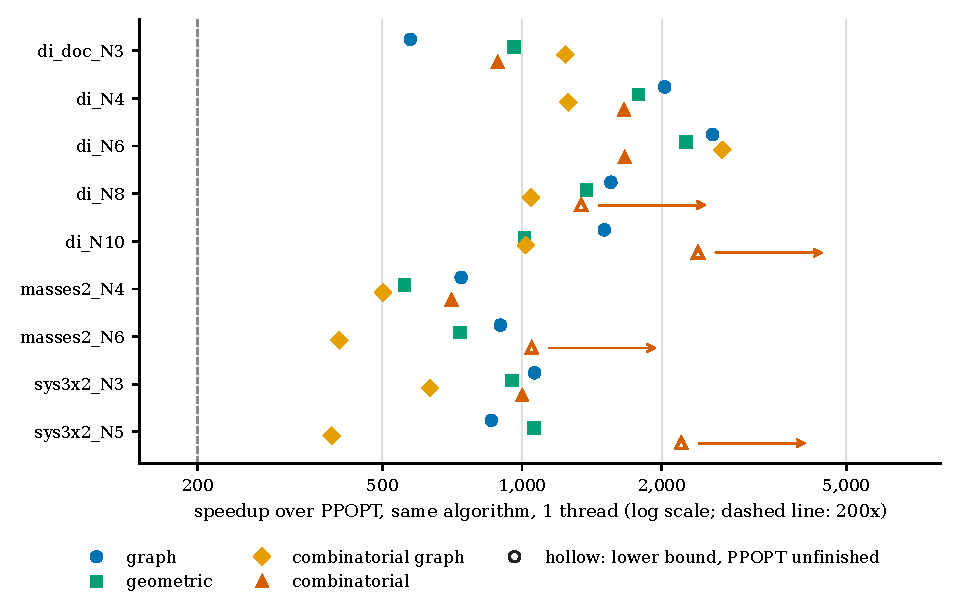
\includegraphics[width=0.86\textwidth]{fig_mpqp_same.pdf}
\caption{Speedup over \ppopt{} for the same algorithm on one thread, per problem. Filled markers: 32 measured pairs. Hollow markers with arrows:
four runs where \ppopt{} did not finish, so the value is a lower bound.}
\label{fig:mpqp}
\end{figure}

\begin{table}[!htbp]
\centering\small\setlength{\tabcolsep}{4pt}
\caption{mpQP, same algorithm, single thread (\code{bench/results/speedup.md}). \ppopt{} time limit 300 s, except two 4 h runs (\code{di\_N10}, \code{sys3x2\_N5} combinatorial). The last column is the region count: equal for \ppopt{} and \rpopt{} on every finished run, and \rpopt{}'s count where \ppopt{} did not finish (marked $>$).}
\label{tab:same}
\begin{tabular}{@{}llrrrr@{}}
\toprule
problem & algorithm & PPOPT & RPOPT (1 thread) & speedup & regions \\
\midrule
\code{di\_N10} & \code{combinatorial} & $>$14,400.00 s & 6.01 s & $>$2,398x & 11 \\
\code{di\_N10} & \code{graph} & 330.9 ms & 220 \textmu s & 1,505x & 11 \\
\code{di\_N10} & \code{geometric} & 112.7 ms & 111 \textmu s & 1,014x & 11 \\
\code{di\_N10} & \code{combinatorial\_graph} & 296.8 ms & 291 \textmu s & 1,020x & 11 \\
\addlinespace[2pt]
\code{di\_N4} & \code{combinatorial} & 621.0 ms & 374 \textmu s & 1,659x & 9 \\
\code{di\_N4} & \code{graph} & 187.5 ms & 92 \textmu s & 2,031x & 9 \\
\code{di\_N4} & \code{geometric} & 89.6 ms & 50 \textmu s & 1,783x & 9 \\
\code{di\_N4} & \code{combinatorial\_graph} & 112.0 ms & 89 \textmu s & 1,259x & 9 \\
\addlinespace[2pt]
\code{di\_N6} & \code{combinatorial} & 14.46 s & 8.7 ms & 1,665x & 11 \\
\code{di\_N6} & \code{graph} & 395.6 ms & 154 \textmu s & 2,577x & 11 \\
\code{di\_N6} & \code{geometric} & 181.6 ms & 80 \textmu s & 2,257x & 11 \\
\code{di\_N6} & \code{combinatorial\_graph} & 600.5 ms & 222 \textmu s & 2,703x & 11 \\
\addlinespace[2pt]
\code{di\_N8} & \code{combinatorial} & $>$300.00 s & 223.5 ms & $>$1,342x & 11 \\
\code{di\_N8} & \code{graph} & 285.6 ms & 184 \textmu s & 1,555x & 11 \\
\code{di\_N8} & \code{geometric} & 126.5 ms & 92 \textmu s & 1,377x & 11 \\
\code{di\_N8} & \code{combinatorial\_graph} & 267.4 ms & 256 \textmu s & 1,046x & 11 \\
\addlinespace[2pt]
\code{di\_doc\_N3} & \code{combinatorial} & 174.6 ms & 197 \textmu s & 887x & 7 \\
\code{di\_doc\_N3} & \code{graph} & 73.0 ms & 127 \textmu s & 575x & 7 \\
\code{di\_doc\_N3} & \code{geometric} & 43.0 ms & 45 \textmu s & 962x & 7 \\
\code{di\_doc\_N3} & \code{combinatorial\_graph} & 100.5 ms & 81 \textmu s & 1,241x & 7 \\
\addlinespace[2pt]
\code{masses2\_N4} & \code{combinatorial} & 9.04 s & 12.8 ms & 705x & 307 \\
\code{masses2\_N4} & \code{graph} & 4.91 s & 6.6 ms & 740x & 307 \\
\code{masses2\_N4} & \code{geometric} & 5.06 s & 9.0 ms & 559x & 307 \\
\code{masses2\_N4} & \code{combinatorial\_graph} & 5.58 s & 11.1 ms & 502x & 307 \\
\addlinespace[2pt]
\code{masses2\_N6} & \code{combinatorial} & $>$300.00 s & 286.1 ms & $>$1,049x & 901 \\
\code{masses2\_N6} & \code{graph} & 39.95 s & 44.4 ms & 899x & 901 \\
\code{masses2\_N6} & \code{geometric} & 24.30 s & 33.0 ms & 736x & 901 \\
\code{masses2\_N6} & \code{combinatorial\_graph} & 46.96 s & 116.2 ms & 404x & 901 \\
\addlinespace[2pt]
\code{sys3x2\_N3} & \code{combinatorial} & 18.04 s & 18.0 ms & 1,001x & 211 \\
\code{sys3x2\_N3} & \code{graph} & 3.09 s & 2.9 ms & 1,065x & 211 \\
\code{sys3x2\_N3} & \code{geometric} & 2.19 s & 2.3 ms & 951x & 211 \\
\code{sys3x2\_N3} & \code{combinatorial\_graph} & 3.43 s & 5.4 ms & 634x & 211 \\
\addlinespace[2pt]
\code{sys3x2\_N5} & \code{combinatorial} & $>$14,400.00 s & 6.53 s & $>$2,206x & 973 \\
\code{sys3x2\_N5} & \code{graph} & 77.54 s & 90.3 ms & 859x & 973 \\
\code{sys3x2\_N5} & \code{geometric} & 18.63 s & 17.5 ms & 1,062x & 973 \\
\code{sys3x2\_N5} & \code{combinatorial\_graph} & 114.23 s & 293.7 ms & 389x & 973 \\
\bottomrule
\end{tabular}
\end{table}

\textbf{Fastest against fastest.} The fastest \ppopt{} algorithm on every problem is \code{geometric}, except \code{masses2\_N4}, where it is \code{graph}. The
fastest \rpopt{} algorithm is \code{mplcp} on 8 of the 9 problems (\code{graph\_exp} on \code{masses2\_N4}). The speedup of fastest over fastest is
753x to 4,062x (Table~\ref{tab:fast}).

\begin{table}[!htbp]
\centering\small
\caption{Fastest serial algorithm per problem, one thread (\code{speedup.md}).}
\label{tab:fast}
\begin{tabular}{@{}lllr@{}}
\toprule
problem & PPOPT's fastest & RPOPT's fastest (1 thread) & speedup \\
\midrule
\code{di\_N10} & \code{geometric} 112.7 ms & \code{mplcp} 63 \textmu s & 1,798x \\
\code{di\_N4} & \code{geometric} 89.6 ms & \code{mplcp} 30 \textmu s & 3,036x \\
\code{di\_N6} & \code{geometric} 181.6 ms & \code{mplcp} 44 \textmu s & 4,167x \\
\code{di\_N8} & \code{geometric} 126.5 ms & \code{mplcp} 53 \textmu s & 2,400x \\
\code{di\_doc\_N3} & \code{geometric} 43.0 ms & \code{mplcp} 27 \textmu s & 1,589x \\
\code{masses2\_N4} & \code{graph} 4.91 s & \code{graph\_exp} 6.5 ms & 755x \\
\code{masses2\_N6} & \code{geometric} 24.30 s & \code{mplcp} 27.5 ms & 884x \\
\code{sys3x2\_N3} & \code{geometric} 2.19 s & \code{mplcp} 1.4 ms & 1,576x \\
\code{sys3x2\_N5} & \code{geometric} 18.63 s & \code{mplcp} 9.5 ms & 1,954x \\
\bottomrule
\end{tabular}
\end{table}

\textbf{Parallel against parallel.} \ppopt{}'s \code{combinatorial\_parallel} uses a process pool; \rpopt{} uses 16 threads. On the seven runs that \ppopt{} finished the speedup is 1,387x to
5,889x, median 2,063x; two runs reached the 300 s limit (Table~\ref{tab:par}).

\begin{table}[!htbp]
\centering\small
\caption{Parallel against parallel (\code{speedup.md}). Regions: equal for \ppopt{} and \rpopt{} on every finished run, \rpopt{}'s count where \ppopt{} did not finish (marked $>$).}
\label{tab:par}
\begin{tabular}{@{}lrrrr@{}}
\toprule
problem & PPOPT (processes) & RPOPT (16 threads) & speedup & regions \\
\midrule
\code{di\_N10} & $>$300.00 s & 571.5 ms & $>$525x & 11 \\
\code{di\_N4} & 1.18 s & 558 \textmu s & 2,110x & 9 \\
\code{di\_N6} & 4.72 s & 3.7 ms & 1,286x & 11 \\
\code{di\_N8} & 66.57 s & 33.5 ms & 1,984x & 11 \\
\code{di\_doc\_N3} & 722.8 ms & 320 \textmu s & 2,260x & 7 \\
\code{masses2\_N4} & 6.76 s & 3.4 ms & 1,960x & 307 \\
\code{masses2\_N6} & 196.24 s & 34.1 ms & 5,755x & 901 \\
\code{sys3x2\_N3} & 12.74 s & 5.1 ms & 2,497x & 211 \\
\code{sys3x2\_N5} & $>$300.00 s & 628.1 ms & $>$478x & 973 \\
\bottomrule
\end{tabular}
\end{table}

\textbf{Time to coverage\busy{}.} Time to cover a given share of $\Theta$ is more relevant than total time when a solver is stopped early. The sweep
(\code{coverage.md}, both sides on the busy machine, so tentative) covers 34 or 35 runs per level. \rpopt{} reaches 99\% and 100\% coverage at least 275x
sooner than \ppopt{} on every run that \ppopt{} reached (Table~\ref{tab:cov}); the one run below 200x at the 90\% level is \code{masses2\_N4}
combinatorial graph (179x), a visit-order effect. Two \ppopt{} runs were stopped at 600 s (\code{di\_N10} combinatorial with 9 of 11 regions built, \code{sys3x2\_N5}
combinatorial with 286 of 973).

\begin{table}[!htbp]
\centering\small
\caption{Time-to-coverage speedup\busy{}, \ppopt{} time over \rpopt{} time, by coverage level (\code{coverage.md}).}
\label{tab:cov}
\begin{tabular}{@{}lrrrr@{}}
\toprule
coverage level & minimum & median & maximum & runs at 200x or more \\
\midrule
50\% & 240x & 1,378x & 5,714x & 35 of 35 \\
90\% & 179x & 1,458x & 5,753x & 33 of 34 \\
99\% & 288x & 1,388x & 6,159x & 34 of 34 \\
100\% & 275x & 1,388x & 8,158x & 34 of 34 \\
all regions & 275x & 1,388x & 8,158x & 34 of 34 \\
total & 276x & 1,438x & 5,946x & 34 of 34 \\
\bottomrule
\end{tabular}
\end{table}

\subsection{mpLP against PPOPT}

\ppopt{}'s geometric and graph solvers leave parts of the feasible set uncovered on most of the degenerate mpLP problems (Table~\ref{tab:gaps}). A
speed comparison with a solver that returns a wrong answer is not meaningful, so \rpopt{}'s fastest solver (\code{mplp\_lex}) is compared with \ppopt{}'s fastest
algorithm that leaves no sampled gap (Table~\ref{tab:mplp}, Figure~\ref{fig:mplp}). The speedup is 836x to 18,028x on the six problems where \ppopt{}
has a gap-free answer. On the seven where it has none within 120 s, the speedup is more than 6,400x (up to more than 305,000x).

\begin{figure}[!htbp]
\centering
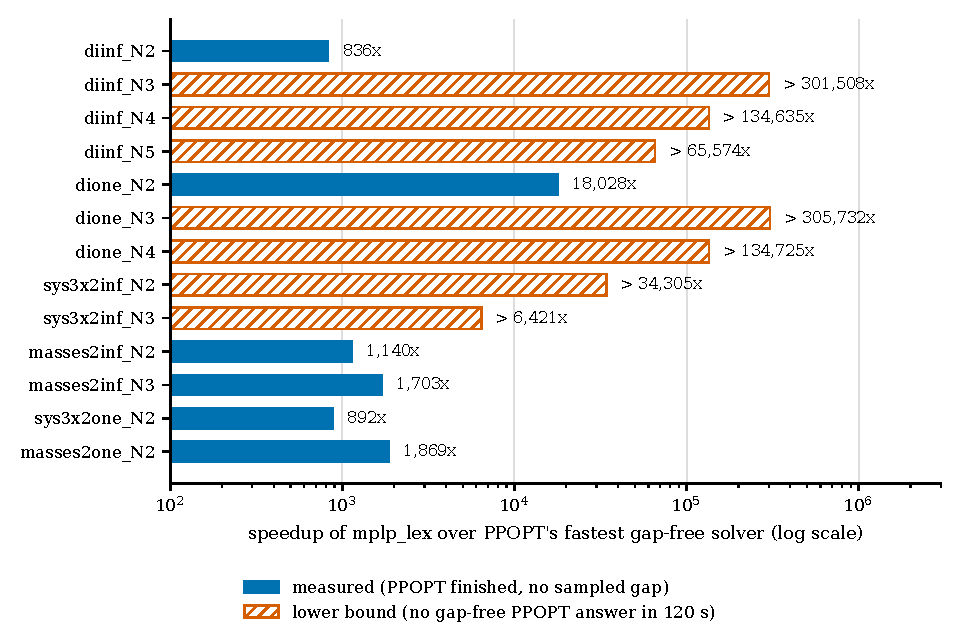
\includegraphics[width=0.86\textwidth]{fig_mplp.pdf}
\caption{mpLP: \rpopt{} \code{mplp\_lex} (one thread) against \ppopt{}'s fastest gap-free solver. Where \ppopt{} produced no gap-free
solution within 120 s, the bar is a lower bound computed with 120 s.}
\label{fig:mplp}
\end{figure}

\begin{table}[!htbp]
\centering\small\setlength{\tabcolsep}{4pt}
\caption{mpLP, \rpopt{} \code{mplp\_lex} against \ppopt{} (\code{mplp\_speedup.md}; regions from \code{mplp\_full.txt}). The percentage in the \ppopt{} geometric
column is the share of sampled feasible parameters not covered by its partition.}
\label{tab:mplp}
\begin{tabular}{@{}l r L{3.9cm} L{3.1cm} r r@{}}
\toprule
problem & regions & PPOPT, fastest gap-free & PPOPT \code{geometric} (sampled gaps) & RPOPT \code{mplp\_lex} & speedup \\
\midrule
\code{diinf\_N2} & 20 & \code{geometric}~144~ms & 144 ms (0.0\%) & 0.17 ms & 836x \\
\code{diinf\_N3} & 31 & none in 120 s & 200 ms (49.8\%) & 0.40 ms & $>$301,508x \\
\code{diinf\_N4} & 39 & none in 120 s & 267 ms (50.4\%) & 0.89 ms & $>$134,635x \\
\code{diinf\_N5} & 47 & none in 120 s & 399 ms (50.4\%) & 1.83 ms & $>$65,574x \\
\code{dione\_N2} & 20 & \code{combinatorial}~3,014~ms & 142 ms (0.3\%) & 0.17 ms & 18,028x \\
\code{dione\_N3} & 30 & none in 120 s & 128 ms (52.7\%) & 0.39 ms & $>$305,732x \\
\code{dione\_N4} & 43 & none in 120 s & 112 ms (76.8\%) & 0.89 ms & $>$134,725x \\
\code{sys3x2inf\_N2} & 152 & none in 120 s & 2,546 ms (0.4\%) & 3.50 ms & $>$34,305x \\
\code{sys3x2inf\_N3} & 504 & none in 120 s & crashes & 18.69 ms & $>$6,421x \\
\code{masses2inf\_N2} & 202 & \code{geometric}~8,121~ms & 8,121 ms (0.0\%) & 7.12 ms & 1,140x \\
\code{masses2inf\_N3} & 1,098 & \code{geometric}~83,868~ms & 83,868 ms (0.0\%) & 49.25 ms & 1,703x \\
\code{sys3x2one\_N2} & 249 & \code{geometric}~4,517~ms & 4,517 ms (0.0\%) & 5.06 ms & 892x \\
\code{masses2one\_N2} & 828 & \code{geometric}~44,642~ms & 44,642 ms (0.0\%) & 23.89 ms & 1,869x \\
\bottomrule
\end{tabular}
\end{table}

\begin{table}[!htbp]
\centering\small
\caption{Coverage of \ppopt{}'s mpLP solutions, sampled at 1,000 random $\theta$ in the parameter box per problem (\code{ppopt\_lp\_coverage.txt}).
``Uncovered samples'' counts feasible samples that fall in no region; ``wrong objective'' counts samples where the stored law's objective differs from the direct LP optimum by more than a relative $10^{-6}$.}
\label{tab:gaps}
\begin{tabular}{@{}lrlrrrr@{}}
\toprule
problem & $n_\theta/n_x/m$ & PPOPT algorithm & regions & uncovered samples & share & wrong objective \\
\midrule
\code{diinf\_N2} & 2/6/24 & \code{geometric} & 18 & 0 of 726 & 0.0\% & 0 \\
\code{diinf\_N3} & 2/9/32 & \code{geometric} & 21 & 347 of 697 & 49.8\% & 0 \\
\code{diinf\_N4} & 2/12/42 & \code{geometric} & 25 & 347 of 689 & 50.4\% & 3 \\
\code{diinf\_N5} & 2/15/52 & \code{geometric} & 34 & 347 of 689 & 50.4\% & 3 \\
\code{dione\_N2} & 2/8/24 & \code{geometric} & 22 & 2 of 726 & 0.3\% & 0 \\
\code{dione\_N3} & 2/12/32 & \code{geometric} & 15 & 367 of 697 & 52.7\% & 0 \\
\code{dione\_N4} & 2/16/42 & \code{geometric} & 11 & 529 of 689 & 76.8\% & 0 \\
\code{sys3x2inf\_N2} & 3/8/40 & \code{geometric} & 168 & 3 of 797 & 0.4\% & 10 \\
\texttt{sys3x2inf\_N3} & 3/12/60 & \texttt{geometric} & \multicolumn{4}{l}{crashes (\texttt{TypeError}, no solution)} \\
\code{masses2inf\_N2} & 4/6/40 & \code{geometric} & 333 & 0 of 535 & 0.0\% & 0 \\
\code{masses2inf\_N3} & 4/9/60 & \code{geometric} & 2,161 & 0 of 472 & 0.0\% & 3 \\
\code{sys3x2one\_N2} & 3/14/40 & \code{geometric} & 399 & 0 of 797 & 0.0\% & 8 \\
\code{masses2one\_N2} & 4/12/40 & \code{geometric} & 1,593 & 0 of 535 & 0.0\% & 3 \\
\code{diinf\_N2} & 2/6/24 & \code{graph} & 30 & 0 of 726 & 0.0\% & 0 \\
\code{diinf\_N3} & 2/9/32 & \code{graph} & 50 & 70 of 697 & 10.0\% & 0 \\
\code{dione\_N2} & 2/8/24 & \code{graph} & 18 & 126 of 726 & 17.4\% & 0 \\
\code{dione\_N3} & 2/12/32 & \code{graph} & 33 & 168 of 697 & 24.1\% & 0 \\
\code{masses2inf\_N2} & 4/6/40 & \code{graph} & 208 & 2 of 535 & 0.4\% & 0 \\
\code{masses2inf\_N2} & 4/6/40 & \code{combinatorial} & 214 & 0 of 535 & 0.0\% & 0 \\
\code{masses2inf\_N2} & 4/6/40 & \code{combinatorial\_graph} & 214 & 0 of 535 & 0.0\% & 0 \\
\code{diinf\_N2} & 2/6/24 & \code{combinatorial} & 30 & 0 of 726 & 0.0\% & 0 \\
\code{dione\_N2} & 2/8/24 & \code{combinatorial} & 22 & 0 of 726 & 0.0\% & 0 \\
\bottomrule
\end{tabular}
\end{table}

\textbf{Same algorithm.} Table~\ref{tab:mplpsame} compares each algorithm with its \ppopt{} counterpart on the 23 pairs where \ppopt{} finished: median 261x,
range 16x to 17,227x. \rpopt{}'s \code{geometric} is 185x to 968x on the 5 problems where \ppopt{}'s geometric covers the feasible set, and 16x to 351x on
the 7 where \ppopt{}'s leaves gaps (and returns fewer regions).

\begin{table}[!htbp]
\centering\small
\caption{mpLP, same algorithm, \rpopt{} one thread against \ppopt{} (\code{mplp\_same\_algorithm.md}).}
\label{tab:mplpsame}
\begin{tabular}{@{}lrrrr@{}}
\toprule
algorithm & pairs & min & median & max \\
\midrule
\code{combinatorial} & 3 & 780x & 922x & 1,475x \\
\code{combinatorial\_graph} & 3 & 213x & 234x & 261x \\
\code{geometric} & 12 & 16x & 188x & 968x \\
\code{graph} & 5 & 1,175x & 2,882x & 17,227x \\
\midrule
all & 23 & 16x & 261x & 17,227x \\
\bottomrule
\end{tabular}
\end{table}

\textbf{Longer horizons.} \code{mplp\_lex} is gap-free with zero errors on all 30 mpLP files (\code{mplp\_full.txt}); its time is 28.7 ms on
\code{diinf\_N10} (62 regions), 2.39 s on \code{masses2one\_N5} (28,336 regions), 206 ms on \code{sys3x2inf\_N5} (2,757 regions). The project README gives
83x for \code{mplp\_lex} against the previous release on \code{diinf\_N10} (2.7 s to 33 ms\busy{}), which was a separate busy-machine measurement
(\code{mplp\_full.txt} has 28.7 ms for the same problem; the difference is run-to-run).

\subsection{Point location}

\textbf{Against \ppopt{}.} \ppopt{}'s numba \code{PointLocation} takes 5.3 to 68.5~\textmu s per query on the nine problems it was timed on. \rpopt{}'s sequential
search (the same algorithm) takes 61 ns to 14.3~\textmu s, and the hash table takes 9 to 32 ns on those nine problems (8 ns on the \code{dinv} problems), 590x to 3,600x faster than \ppopt{} (Figure~\ref{fig:pl}). The
dinv problems have no \ppopt{} run.

\begin{figure}[!htbp]
\centering
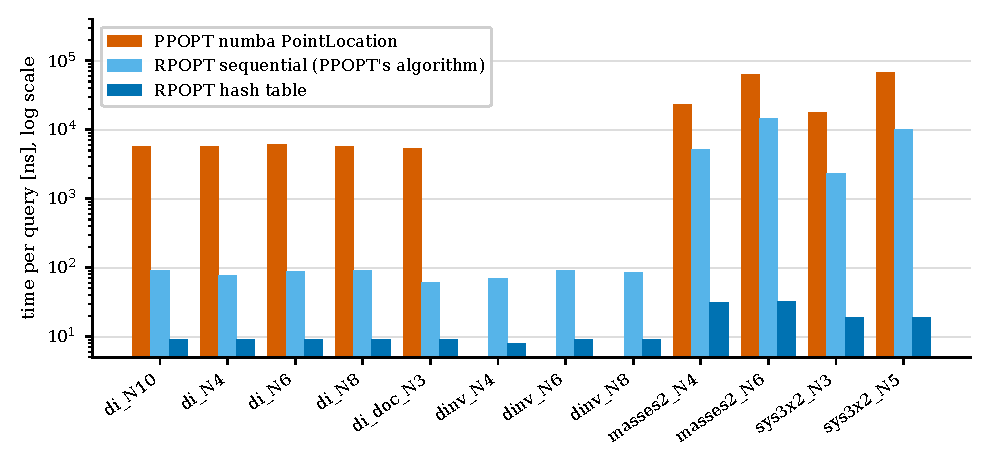
\includegraphics[width=0.88\textwidth]{fig_pl.pdf}
\caption{Point location time per query on the 12 mpQP problems: \ppopt{}'s numba \code{PointLocation}, \rpopt{}'s port of the same sequential algorithm, and
\rpopt{}'s fastest method, the hash table (storage limit chosen per problem; \code{speedup.md}). Log scale. No \ppopt{} bars for the \code{dinv} problems.}
\label{fig:pl}
\end{figure}

\textbf{All methods on the benchmark.} Table~\ref{tab:plmethods} lists every locator on the nine original problems, 100,000 uniform queries
(\code{point\_location.md}; the run did not record machine load, and its hash table column is the fixed ``16R boxes'' grid, so it is slower than the storage-limited table
of Figure~\ref{fig:pl} on the larger problems). The hash table is fastest on every problem. A linear machine exists only for facet-to-facet
partitions; for \code{masses2\_N4}, \code{masses2\_N6}, \code{sys3x2\_N3} and \code{sys3x2\_N5} the partitions contain 118, 286, 6 and 22 non-facet-to-facet
facets, so none exists (an argmax of affine functions is always face-to-face).

\newcommand{\linmachnote}{linear machine, ns per query: \code{di\_N10} 29, \code{di\_N4} 28, \code{di\_N6} 30, \code{di\_N8} 29, \code{di\_doc\_N3} 25; none exists on \code{masses2\_N4}, \code{masses2\_N6}, \code{sys3x2\_N3}, \code{sys3x2\_N5}}
\begin{table}[!htbp]
\centering\small\setlength{\tabcolsep}{4pt}
\caption{Point location, ns per query, 100,000 uniform queries. All methods agree with sequential search on every query. Omitted column: \linmachnote.}
\label{tab:plmethods}
\begin{tabular}{@{}lrrrrrrrrr@{}}
\toprule
problem & $n_\theta/n_x/m$ & regions & seq. & seq. early & BST & multiway & descr. & hash & YANN \\
\midrule
\code{di\_N10} & 2/10/42 & 11 & 74 & 33 & 41 & 36 & 41 & 22 & 76 \\
\code{di\_N4} & 2/4/18 & 9 & 65 & 30 & 35 & 31 & 38 & 22 & 65 \\
\code{di\_N6} & 2/6/26 & 11 & 74 & 33 & 41 & 36 & 41 & 22 & 74 \\
\code{di\_N8} & 2/8/34 & 11 & 74 & 33 & 40 & 36 & 41 & 21 & 76 \\
\code{di\_doc\_N3} & 2/9/20 & 7 & 51 & 28 & 33 & 28 & 35 & 21 & 48 \\
\code{masses2\_N4} & 4/4/40 & 307 & 4,773 & 1,252 & 180 & 135 & 1,038 & 65 & 4,670 \\
\code{masses2\_N6} & 4/6/60 & 901 & 13,795 & 5,167 & 233 & 165 & 4,070 & 73 & 13,664 \\
\code{sys3x2\_N3} & 3/6/30 & 211 & 1,956 & 784 & 120 & 96 & 667 & 37 & 1,931 \\
\code{sys3x2\_N5} & 3/10/50 & 973 & 8,999 & 4,338 & 147 & 113 & 3,476 & 46 & 9,007 \\
\bottomrule
\end{tabular}
\end{table}

\textbf{Trees against grids, 2 to 10 parameters\busy{}.} \code{examples/pl\_dim\_sweep.rs} builds locators for random mpQPs and spring chains with 11 to 7,919 regions
(file \code{pl\_dim\_sweep\_busy\_machine.txt}). Table~\ref{tab:plsweep} shows a selection. At equal storage no tree beat the hash table on volume-uniform or closed-loop queries up to 8
parameters. The hash table is 5x to 20x faster at 2 to 4 parameters and 3x to 10x faster at 5 to 8 (project README summary of the sweep). Trees grow 1.4x
to 2x deeper than $\log_2$ of the region count, because regions that straddle a cut are copied into both branches. Trees win only on region-uniform queries at 4 to 6 parameters, where many tiny regions crowd
a few grid cells. The raw file also records nonzero mismatch counts (7 to 68 in several tree variants, 21 for the 64 MB hash table on one 8-parameter instance) from before the
bug fixed afterwards (\S\ref{sec:correctness}); the 8 MB hash table of the table has 0 mismatches. At 8 parameters the BST (truncated build) is no
faster than a sequential scan (26,754 against 24,559 ns on a 1,204-region problem).

\begin{table}[!htbp]
\centering\small\setlength{\tabcolsep}{4pt}
\caption{Point location by parameter count\busy{}, ns per volume-uniform query (selected instances). An asterisk marks a tree whose build was truncated at 45 s. Instance names: \code{qp:$n_x$:$n_\theta$:$m$:seed} are random mpQPs, \code{mass:k:n} spring chains. The mismatch column for the 8 MB hash table is omitted: it is 0 on every listed instance.}
\label{tab:plsweep}
\begin{tabular}{@{}lrrrrrr@{}}
\toprule
instance & $n_\theta$ & regions & sequential & BST & optimized tree & hash table, 8 MB \\
\midrule
\code{di\_N10} & 2 & 11 & 34 & 44 & 40 & 9 \\
\code{qp:8:3:100:2} & 3 & 2,236 & 19,728 & 148 & 142 & 7 \\
\code{masses2\_N6} & 4 & 901 & 5,758 & 269 & 230 & 45 \\
\code{qp:8:4:60:1} & 4 & 4,639 & 110,865 & 344 & 925* & 8 \\
\code{qp:6:5:40:1} & 5 & 7,919 & 83,398 & 41,722* & 1,579* & 86 \\
\code{qp:4:6:14:1} & 6 & 841 & 10,883 & 4,564* & 978* & 109 \\
\code{mass:3:3} & 6 & 955 & 18,498 & 6,339* & 1,306* & 282 \\
\code{qp:4:8:14:1} & 8 & 1,204 & 24,559 & 26,754* & 17,118* & 1,660 \\
\bottomrule
\end{tabular}
\end{table}

\textbf{Larger problems\busy{}.} On the large suite's POP problems, the geometric mean over problems is 4,499 ns (uniform) and 4,407 ns (closed-loop trajectory) for
\ppopt{}'s sequential algorithm, 1,028 and 416 ns for sequential with early exit, 93 and 73 ns for the BST, 82 and 68 for the multiway tree, 67 and 41 for the hash table. The
BST and multiway trees were skipped on partitions of more than 3,000 regions (\code{--bst-max-regions}) and the partition geometry, which the other locators need, on partitions of more than 15,000
(\code{--geom-max-regions}), where only the sequential and YANN locators remain. The walking methods start from the previous answer; on closed-loop
trajectories run 2x to 5x slower than the hash table on the benchmark problems (README).

\subsection{Horizon scaling\busy{}}
\label{sec:scaling}

\code{bench/results/scaling.txt} times every exact solver at increasing horizons on the double integrator (11 regions at every horizon, to $N=30$), two masses (to $N=8$, 2,837 regions)
and the 3-state, 2-input system (to $N=7$, 2,095 regions). All values are from a busy machine, so absolute values are noisy. The combinatorial algorithm grows by a factor of
about 5 to 6 per added horizon step on the double integrator (243 ms at $N=8$, 6.3 s at $N=10$, 221 s at $N=12$), and is skipped beyond $N=12$ and for \code{sys3x2} at $N=7$. The \code{dp} column (active-set dynamic programming) failed at $N=25$ because it supports at most 128 constraints, and was skipped at $N=30$.
Every other solver grows slowly. \code{mplcp} is the fastest at every point listed in Table~\ref{tab:scaling}; in the full file, \code{graph} is faster on \code{masses2} at $N=4$ and $5$ (10.4 and 23.0 ms against 14.5 and 35.4 ms). Every timed row in the file reports the same region count as the reference solver (column \code{same}).

\begin{figure}[!htbp]
\centering
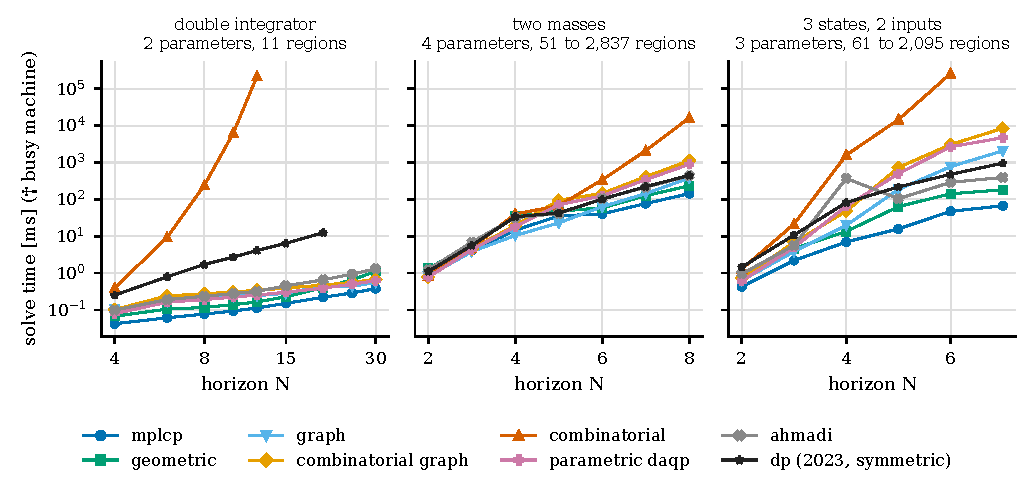
\includegraphics[width=\textwidth]{fig_scaling.pdf}
\caption{Solve time of every exact solver against the horizon\busy{}. Missing points: combinatorial is skipped at large horizons, and \code{dp} fails or is skipped beyond $N=20$ on the double integrator.}
\label{fig:scaling}
\end{figure}

\begin{table}[!htbp]
\centering\small\setlength{\tabcolsep}{4pt}
\caption{Solve time in ms at selected horizons\busy{} (\code{scaling.txt}); ``--'' skipped, ``fail'' did not complete. \code{pdaqp} is \code{parametric\_daqp}.}
\label{tab:scaling}
\begin{tabular}{@{}lrrrrrrrrr@{}}
\toprule
instance & regions & mplcp & geom. & graph & comb. graph & pdaqp & ahmadi & dp & comb. \\
\midrule
\code{di\_N10} & 11 & 0.093 & 0.139 & 0.235 & 0.307 & 0.222 & 0.278 & 2.71 & 6,328 \\
\code{di\_N12} & 11 & 0.113 & 0.164 & 0.243 & 0.338 & 0.253 & 0.318 & 4.08 & 221,065 \\
\code{di\_N20} & 11 & 0.220 & 0.401 & 0.442 & 0.471 & 0.388 & 0.651 & 12.4 & -- \\
\code{di\_N30} & 11 & 0.378 & 1.11 & 0.557 & 0.676 & 0.618 & 1.30 & -- & -- \\
\code{masses2\_N6} & 901 & 40.3 & 58.9 & 63.2 & 145 & 125 & 103 & 101 & 338 \\
\code{masses2\_N8} & 2,837 & 143 & 234 & 378 & 1,122 & 892 & 433 & 448 & 16,325 \\
\code{sys3x2\_N5} & 973 & 15.7 & 63.4 & 186 & 731 & 497 & 104 & 218 & 14,561 \\
\code{sys3x2\_N7} & 2,095 & 66.8 & 182 & 2,076 & 8,460 & 4,716 & 393 & 958 & -- \\
\bottomrule
\end{tabular}
\end{table}

\subsection{Large suite\busy{}}

The large suite (131 problems, 1 to 10 parameters, busy machine) tests scale and robustness. Table~\ref{tab:large} summarizes the exact
solvers. \code{mplcp} is the fastest, at a geometric mean of 0.76 of \code{graph}'s time; it solves 124 problems and times out on 7. The timeout is a per-solve cap, so timed-out problems are not in the means.
\code{combinatorial} was run only on 79 problems (the others appear as ``-'' in \code{large.md}) and never timed out.

\begin{table}[!htbp]
\centering\small
\caption{Large suite summary\busy{}: problems solved, timed out and geometric-mean time relative to \code{graph} on the problems both solved (\code{large.md}).}
\label{tab:large}
\begin{tabular}{@{}lrrr@{}}
\toprule
algorithm & solved & timed out & geometric mean time vs \texttt{graph} \\
\midrule
\code{combinatorial} & 79 & 0 & 1.57 \\
\code{geometric} & 119 & 12 & 1.02 \\
\code{graph} & 124 & 7 & 1.00 \\
\code{combinatorial\_graph} & 122 & 9 & 1.03 \\
\code{ahmadi} & 120 & 11 & 1.17 \\
\code{mplcp} & 124 & 7 & 0.76 \\
\bottomrule
\end{tabular}
\end{table}

\textbf{Active-set disagreements.} On 59 of the 131 problems, the algorithms do not return the same set of active sets, and on 34 of the 44 problems with at
least 3,000 regions the region counts differ between algorithms (for example 3,638, 3,642 and 3,643 on \code{masses3\_N4}, and 37,937 to 38,469 on \code{masses3\_N7}). On 22
problems, the 2,000-sample check reports gaps, overlaps or wrong laws for at least one algorithm. Some of these are small POP problems (\code{pop\_001}, \code{pop\_052},
\code{pop\_071}, \code{pop\_081}) that the report does not analyse. I have not found the cause of the disagreement on the large MPC problems. It is open
(\S\ref{sec:limits}). The large-suite file predates the point location fixes of \S\ref{sec:correctness}, so its trajectory mismatch counts for the trees (for example 16 on \code{masses2\_N8}) are not current.

\subsection{Release-to-release}

Against frozen binaries of commit \code{778cdb9} (one thread, alternating runs), the median is 3.48x on mpLP (54 pairs, range 0.97x to 1,269x, none below 0.95x) and 1.10x on mpQP
(60 pairs, range 0.98x to 1.79x, none below 0.95x). Figure~\ref{fig:score} shows every pair and Table~\ref{tab:score} the per-algorithm summary.

\begin{figure}[!htbp]
\centering
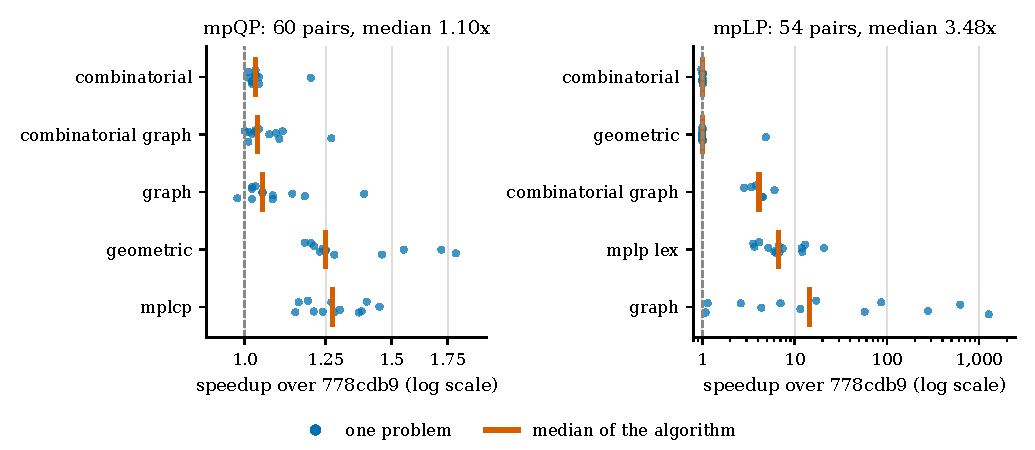
\includegraphics[width=\textwidth]{fig_scoreboard.pdf}
\caption{Release-to-release speedup of \rpopt{} over commit \code{778cdb9}, one point per (problem, algorithm) pair; vertical bars mark the median of each algorithm. Dashed line: 1x.}
\label{fig:score}
\end{figure}

\begin{table}[!htbp]
\centering\small
\caption{Release-to-release summary by algorithm (\code{scoreboard\_vs\_778cdb9\_*.md}). Pairs where the baseline did not finish are excluded from the medians. A dash means the algorithm has no pairs in that problem class.}
\label{tab:score}
\begin{tabular}{@{}lrrrrrrr@{}}
\toprule
 & \multicolumn{3}{c}{mpQP (12 problems)} & & \multicolumn{3}{c}{mpLP (timed pairs)} \\
\cmidrule(r){2-4}\cmidrule(l){6-8}
algorithm & min & median & max & & min & median & max \\
\midrule
\code{combinatorial} & 1.01x & 1.03x & 1.20x & & 0.97x & 1.01x & 1.01x \\
\code{combinatorial\_graph} & 1.00x & 1.04x & 1.27x & & 2.83x & 4.10x & 6.04x \\
\code{geometric} & 1.18x & 1.25x & 1.79x & & 0.98x & 1.00x & 4.86x \\
\code{graph} & 0.98x & 1.05x & 1.39x & & 1.08x & 14.33x & 1,269.16x \\
\code{mplcp} & 1.15x & 1.27x & 1.45x & & -- & -- & -- \\
\code{mplp\_lex} & -- & -- & -- & & 3.56x & 6.70x & 20.75x \\
\bottomrule
\end{tabular}
\end{table}

\textbf{mpLP.} The gain comes from the repaired graph solver and from \code{mplp\_lex}: \code{mplp\_lex} 6.7x (median; \code{diinf\_N5} 20.8x), \code{graph} 14.3x (up to 1,269x on
\code{dione\_N4}, where the old graph solver left gaps), \code{combinatorial\_graph} 4.1x. The old \code{graph} partitions had gaps on all 12 timed mpLP pairs (4 to 879 uncovered samples of 2,000, for example 446 on \code{diinf\_N2}); the new ones have none, so \code{graph}'s ratio mixes a speed change and a different (complete) region set. \code{combinatorial} and \code{geometric} are essentially unchanged (median 1.01x and 1.00x), except \code{geometric} on \code{dione\_N4} (4.86x). Three baseline runs timed out and finished with the current code (\code{masses2inf\_N3} and \code{masses2one\_N2} combinatorial graph, \code{sys3x2inf\_N3} graph).

\textbf{mpQP.} \code{mplcp} gains 1.27x (1.15x to 1.45x) and \code{geometric} 1.25x (1.18x to 1.79x). \code{graph}, \code{combinatorial\_graph} and \code{combinatorial} gain only 1.03x to 1.05x, because their time is in rank tests,
control-law and row assembly, and candidate enumeration rather than in LPs (\S\ref{sec:census}). \textbf{The 1.5x target was not met on mpQP.}

\subsection{Where the LP solves and time go}
\label{sec:census}

\code{lp\_census.md} is a measurement-only study (no algorithm changed) that counts every LP and QP by purpose on the baseline
(\code{778cdb9}) and asks whether a shared improvement of region construction could reach 1.5x. Counts are exact; times were taken at load 50 to 100 and are noisy\busy{}.
Table~\ref{tab:census} shows the overview for the two largest mpQP problems and one mpLP problem.

\begin{table}[!htbp]
\centering\small\setlength{\tabcolsep}{4pt}
\caption{LP census (\code{lp\_census.md}). LPs are counted per solve; LP time share is of total solve time\busy{}.}
\label{tab:census}
\begin{tabular}{@{}lrlrrrrr@{}}
\toprule
problem & $n_\theta/n_x/m$ & algorithm & regions & LPs & LPs per region & QPs & LP time / solve$^\dagger$ \\
\midrule
\code{masses2\_N6} & 4/6/60 & \code{geometric} & 901 & 31,611 & 35.1 & 7,347 & 77\% \\
\code{masses2\_N6} & 4/6/60 & \code{graph} & 901 & 48,903 & 54.3 & 100 & 29\% \\
\code{masses2\_N6} & 4/6/60 & \code{graph\_exp} & 901 & 52,961 & 58.8 & 100 & 65\% \\
\code{masses2\_N6} & 4/6/60 & \code{combinatorial\_graph} & 901 & 157,087 & 174.3 & 1 & 42\% \\
\code{masses2\_N6} & 4/6/60 & \code{mplcp} & 901 & 4,469 & 5.0 & 1 & 2\% \\
\code{masses2\_N6} & 4/6/60 & \code{combinatorial} & 901 & 342,759 & 380.4 & 0 & 42\% \\
\addlinespace[2pt]
\code{sys3x2\_N5} & 3/10/50 & \code{geometric} & 973 & 22,179 & 22.8 & 5,511 & 44\% \\
\code{sys3x2\_N5} & 3/10/50 & \code{graph} & 973 & 88,226 & 90.7 & 100 & 23\% \\
\code{sys3x2\_N5} & 3/10/50 & \code{graph\_exp} & 973 & 111,492 & 114.6 & 100 & 21\% \\
\code{sys3x2\_N5} & 3/10/50 & \code{combinatorial\_graph} & 973 & 358,390 & 368.3 & 1 & 17\% \\
\code{sys3x2\_N5} & 3/10/50 & \code{mplcp} & 973 & 1,515 & 1.6 & 1 & 9\% \\
\code{sys3x2\_N5} & 3/10/50 & \code{combinatorial} & 973 & 7,543,221 & 7,752.5 & 0 & 40\% \\
\addlinespace[2pt]
\code{diinf\_N4} & 2/12/42 & \code{geometric} & 39 & 2,284 & 58.6 & 0 & 52\% \\
\code{diinf\_N4} & 2/12/42 & \code{mplp\_lex} & 39 & 982 & 25.2 & 0 & 2\% \\
\bottomrule
\end{tabular}
\end{table}

\textbf{Verdict.} Shared, LP-only region-construction work cannot give every algorithm 1.5x. If the LPs inside region construction were cut by 100\%,
the Amdahl bound $1/(1-f)$ would be 1.63x and 1.10x for \code{geometric} (\code{masses2\_N6} and \code{sys3x2\_N5}), 1.26x and 1.15x for \code{graph}, 1.28x and 1.05x for
\code{combinatorial\_graph}, 1.08x and 1.00x for \code{combinatorial}, and 1.07x and 1.05x for \code{geometric} on the mpLPs \code{diinf\_N4} and \code{diinf\_N6}. Only \code{graph\_exp} on \code{masses2\_N6} clears 1.5x,
and that figure rests on a bounding-box time that varied 3.5x between runs with identical LP counts. The reasons per algorithm:
\begin{itemize}
  \item \textbf{geometric.} LP and QP are 77\% (\code{masses2\_N6}) and 44\% (\code{sys3x2\_N5}) of the time. Neighbour search (facet-centre LPs and
    7,346 facet-step QPs) is the largest piece, 38\% and 35\%, and 69\% of facet steps end on an already indexed active set. This is the one lever that could reach 1.5x.
  \item \textbf{graph, combinatorial graph.} LP is only 29\% and 23\% (graph) and 42\% and 17\% (combinatorial graph) of the time. The rest is rank tests, control-law
    and row assembly, candidate generation and hashing; the combinatorial graph generates 343,882 (\code{masses2\_N6}) and 1,237,377 (\code{sys3x2\_N5}) duplicate neighbour entries for 901 and 973 regions.
  \item \textbf{combinatorial.} Feasibility LPs are 86\% to 100\% of its LPs and 34\% to 40\% of its time (\code{masses2\_N6}, \code{sys3x2\_N5}), and 57\% to 80\% come back infeasible even after the pruning list removed 84\% of the candidates.
    Removing every feasibility LP gives 1.51x to 1.65x at best.
  \item \textbf{mplcp and mplp\_lex.} LP is 2\% to 15\% (\code{mplcp}) and 0\% to 2\% (\code{mplp\_lex}) of the time. Their time is in pivoting and the non-LP half of region construction.
\end{itemize}
Avoiding duplicate region builds saves nothing: every region build in the graph-type algorithms is kept (901 builds for 901 regions), and the only wasted builds are the combinatorial
algorithm's 22,888 empty-region tests, about 3\% of its time.

\subsection{Multi-threading\busy{}}
\label{sec:threads}

The parallel algorithms reproduce the serial region set at every thread count (\code{thread\_scaling.md}). On the larger problems the combinatorial algorithm scales to 9.5x to 10.4x
at 16 threads against 1 on the three longest solves (\code{di\_N8}, \code{masses2\_N6}, \code{sys3x2\_N5}) and 5.5x to 6.2x on the other two (the machine has 12 performance and 4 efficiency cores). The geometric, graph and combinatorial graph variants reach 2.1x to 6.6x
on the four other problems, and the smallest problem (\code{di\_N8}) does not benefit: the whole solve takes under 1 ms, and \code{graph\_parallel} and \code{geometric\_parallel} are slower than one thread (0.6x and 0.5x). \code{mplcp\_parallel}
falls back to serial code on small problems and, per the README, is reported in the README to scale to 4.7x on 8 threads on the larger problems.

\begin{table}[!htbp]
\centering\small\setlength{\tabcolsep}{4pt}
\caption{Thread scaling\busy{}: solve time in ms (\code{thread\_scaling.md}). ``serial'' is the serial algorithm on one thread; the next columns are the parallel code at the given thread count.}
\label{tab:threads}
\begin{tabular}{@{}llrrrrrrr@{}}
\toprule
problem & algorithm & serial & 1 & 2 & 4 & 8 & 16 & 16 vs 1 \\
\midrule
\code{di\_N8} & \code{combinatorial} & 957.6 & 966.9 & 504.7 & 263.6 & 146.1 & 102.0 & 9.5$\times$ \\
\code{di\_N8} & \code{graph} & 0.3 & 0.4 & 0.3 & 0.3 & 0.5 & 0.7 & 0.6$\times$ \\
\code{di\_N8} & \code{combinatorial\_graph} & 0.6 & 0.6 & 0.5 & 0.3 & 0.5 & 0.7 & 1.0$\times$ \\
\code{di\_N8} & \code{geometric} & 0.1 & 0.2 & 0.2 & 0.2 & 0.3 & 0.4 & 0.5$\times$ \\
\addlinespace[2pt]
\code{masses2\_N4} & \code{combinatorial} & 29.6 & 29.4 & 15.4 & 8.1 & 5.3 & 4.8 & 6.2$\times$ \\
\code{masses2\_N4} & \code{graph} & 12.8 & 13.5 & 7.4 & 4.5 & 3.4 & 3.5 & 3.9$\times$ \\
\code{masses2\_N4} & \code{combinatorial\_graph} & 22.6 & 23.0 & 12.4 & 7.2 & 4.9 & 4.9 & 4.7$\times$ \\
\code{masses2\_N4} & \code{geometric} & 15.6 & 15.5 & 8.3 & 4.8 & 3.6 & 3.5 & 4.5$\times$ \\
\addlinespace[2pt]
\code{masses2\_N6} & \code{combinatorial} & 936.3 & 935.8 & 483.9 & 248.9 & 132.3 & 89.9 & 10.4$\times$ \\
\code{masses2\_N6} & \code{graph} & 75.2 & 94.3 & 50.4 & 29.0 & 19.1 & 16.9 & 5.6$\times$ \\
\code{masses2\_N6} & \code{combinatorial\_graph} & 249.8 & 253.0 & 137.0 & 76.3 & 47.5 & 38.2 & 6.6$\times$ \\
\code{masses2\_N6} & \code{geometric} & 62.8 & 65.3 & 34.4 & 18.8 & 11.7 & 10.0 & 6.5$\times$ \\
\addlinespace[2pt]
\code{sys3x2\_N3} & \code{combinatorial} & 52.3 & 51.6 & 27.2 & 14.5 & 10.5 & 9.4 & 5.5$\times$ \\
\code{sys3x2\_N3} & \code{graph} & 4.9 & 5.8 & 3.4 & 2.2 & 2.3 & 2.7 & 2.1$\times$ \\
\code{sys3x2\_N3} & \code{combinatorial\_graph} & 11.1 & 11.4 & 6.2 & 3.7 & 3.0 & 3.5 & 3.2$\times$ \\
\code{sys3x2\_N3} & \code{geometric} & 4.7 & 4.8 & 2.9 & 1.8 & 2.0 & 2.2 & 2.2$\times$ \\
\addlinespace[2pt]
\code{sys3x2\_N5} & \code{combinatorial} & 23,580.0 & 23,721.8 & 12,491.1 & 6,357.6 & 3,386.4 & 2,309.9 & 10.3$\times$ \\
\code{sys3x2\_N5} & \code{graph} & 143.4 & 351.6 & 191.1 & 105.5 & 68.7 & 55.7 & 6.3$\times$ \\
\code{sys3x2\_N5} & \code{combinatorial\_graph} & 629.1 & 646.4 & 357.9 & 209.5 & 137.8 & 110.2 & 5.9$\times$ \\
\code{sys3x2\_N5} & \code{geometric} & 37.6 & 39.9 & 22.0 & 11.9 & 9.2 & 8.3 & 4.8$\times$ \\
\bottomrule
\end{tabular}
\end{table}

% =====================================================================================
\section{Correctness findings and bugs fixed}
\label{sec:correctness}

\subsection{Degenerate mpLPs: gaps in \ppopt{} and in the port}

\begin{itemize}
  \item \textbf{Facet stepping on degenerate problems} (\ppopt{}'s version and the original port) can leave holes: 16\% of the parameter set on a 3D degenerate vertex, and no regions at
    all on another case. There were three causes: zero-width facets are skipped; a degenerate step point picks an arbitrary basis; and a facet with several neighbours is stepped across only
    once. \rpopt{} picks a canonical basis at degenerate points and completes suspect facets~\cite{spjotvold2006facet}. Results on non-degenerate problems are unchanged. On \ppopt{}, the sampled gap of
    \code{geometric} is 49.8\% to 76.8\% on five mpLPs (\code{diinf\_N3}, \code{N4}, \code{N5}, \code{dione\_N3}, \code{N4}), 0.3\% and 0.4\% on two more, and the solver crashes on \code{sys3x2inf\_N3} (Table~\ref{tab:gaps}).
  \item \textbf{Graph solvers on degenerate mpLPs.} The pruning list blocked the one-pivot step to a neighbouring basis, and the search never left lower-dimensional optimal bases. This was partly a
    bug in the port and partly inherited from \ppopt{}, whose graph solver leaves 10.0\%, 17.4\% and 24.1\% of the sampled parameters uncovered on \code{diinf\_N3}, \code{dione\_N2} and \code{dione\_N3} (and 0.4\% on \code{masses2inf\_N2}; Table~\ref{tab:gaps}).
    \rpopt{} generates the pivot swaps directly and finishes with a facet-completion pass, so the partition is gap-free. The previous \rpopt{} release shows the same
    defect (gaps of 4 to 879 samples of 2,000 on all 12 timed mpLP pairs; the scoreboard file records them).
  \item \textbf{Degenerate-vertex basis enumeration in \code{geometric}.} Enumerating all bases at a degenerate vertex is exponential; when the count exceeds 1,000, an LP over the multiplier polyhedron picks the canonical basis. \code{diinf\_N8} went from 2.1 s to 50 ms
    (busy machine\busy{}).
\end{itemize}

\subsection{Other porting bugs and deliberate differences}

\begin{itemize}
  \item \textbf{Dense LP false infeasibility} from 48 variables up (anti-cycling rule switched on too early). Fixed; decisions now match Clarabel up to 192 variables.
  \item \textbf{Parameter bounding box.} When constraint processing drops parameter bounds as redundant, the box now falls back to the feasible parameter set.
  \item \textbf{Skipped \code{check\_optimality} LP.} \ppopt{}'s combinatorial algorithm runs it before building each region; under LICQ its answer equals the region's nonemptiness, which region construction already checks.
  \item \textbf{Visit order.} \ppopt{}'s combinatorial graph pops candidates from a Python set, in hash order. \rpopt{} uses breadth first, which finds the large regions early; the explored set is the same.
  \item \textbf{Other conventions.} \code{Solution.is\_overlapping} is set only for mpLPs and non-convex mpQPs (\ppopt{} sets it for every mpQP); \code{get\_independent\_rows} keeps the last equality row when it is independent; duals use the standard sign convention ($Qx+c+A^\top\lambda=0$, $\lambda\ge0$).
\end{itemize}

\subsection{Point location}

\begin{itemize}
  \item \textbf{Boundary tie rule.} \ppopt{} returns the first region within its tolerance, or the lowest objective among those regions for overlapping solutions. Near a facet, that can be a neighbour whose law, extended
    past its boundary, is infeasible and looks better than the optimum. \rpopt{} prefers a region that contains the parameter strictly; every locator except the descriptor function and YANN shares the rule (\code{pick\_strict\_first}).
  \item \textbf{Certified interior checks.} The dimension sweep showed 7 to 68 mismatches on instances with 6 to 8 parameters. The cause was the Chebyshev LP that decides whether a region meets a hash cell or a tree cut with positive volume: it
    returned radius 0 for thin or badly scaled polytopes that do have an interior (radii up to 28 times too small on data of magnitude 38). Now a region is dropped only when a known-point hint, the plain LP and a recentred LP all say no (and, in the second fix, a verified multiplier certificate), and regions whose vertex lists may be incomplete are marked thin: trees never classify them
    from vertices and the hash table bounds them by coordinate LPs. After the fix the mass chain \code{mass:3:3}, which had mismatches in every tree variant, has 0 for all trees and tables, and \code{tests/pl\_agreement.rs} checks that all 12 locators agree with \code{Solution::\allowbreak{}get\_region} on
    24,000 uniform and near-facet queries at 6 and 8 parameters.
  \item \textbf{Hash table up to 16 parameters.} The hash table now supports 1 to 16 parameters; \code{try\_with\_storage\_limit} returns an error beyond that.
  \item \textbf{One tolerance.} \code{Solution} and every locator use one point location tolerance, 1e-9 (\ppopt{} uses 1e-5). Shared facets of neighbouring regions agree to about 1e-13 (at worst 1e-10), while at 1e-5 a point just outside the partition can receive a region whose extended law violates the constraints by up to 0.16.
\end{itemize}

\subsection{Comparison with the authors' DAQP implementation}

Per the project README, \code{parametric\_daqp} is 1.5x to 2.9x faster than \code{pdaqp} 0.7.1 (ParametricDAQP.jl, the authors' implementation of \cite{arnstrom2024high}) on the larger problems,
and \code{geometric} is about 14x faster than \code{pdaqp} on \code{sys3x2\_N5} (46 ms against 645 ms). On that problem \code{pdaqp} returns 967 regions against 973. The 6 it drops are thin but real:
direct QP solves confirm them, its default \code{lowdim\_tol} discards them, and with \code{lowdim\_tol = 0} it returns all 973. These \code{pdaqp} figures are from the README; I found no committed result file for them in
\code{bench/results}.

% =====================================================================================
\section{Limitations and open items}
\label{sec:limits}

\begin{enumerate}
  \item \textbf{The mpQP 1.5x target was not met.} The measured median is 1.10x, and the LP census shows that no LP-only change can reach it for the graph and combinatorial algorithms (\S\ref{sec:census}).
    The one lever that could, for \code{geometric}, is neighbour search by inspection (an upper bound of 1.53x to 1.80x), but it was not built. Reading the \code{mplcp} law from the pivot tableau gave only about 2\%. It is now the default; its coefficients agree with
    the KKT solve to about 6e-9 relative but are not bit-identical, and \code{mplcp::set\_tableau\_law(false)} restores the KKT solve.
  \item \textbf{Remaining region differences on large problems.} A diff of the algorithms' partitions on six large problems found three defects, now fixed: \code{mplcp} missed real regions when facet rows were large (an absolute zero-row tolerance), \code{combinatorial\_graph} kept noise slivers and two rank-deficient regions from its incremental update, and redundancy removal could drop both rows of a near-duplicate pair. What remains are thin regions (Chebyshev radius below 1e-6) and three small regions on \code{masses3\_N5} (radius 1.5e-6 to 2.4e-6) found by \code{graph} only. The benchmark's same-active-set check should compare partitions by sampled coverage instead.
  \item \textbf{Exact duplicate rows in mpMILP subproblems.} \code{graph} returns no region on one mpMILP root relaxation with exactly duplicated rows (ignored test \code{dump\_repro}).
  \item \textbf{Busy-machine data.} The large suite, horizon scaling, point location sweep, coverage sweep and thread scaling should be rerun on a quiet machine before their absolute values are quoted; the large suite also predates the point location fixes.
  \item \textbf{Scope.} The symbolic modeler, the code generators and the 1-D overlap reduction for mpMILP are not ported. The dynamic programming solver is limited to 128 constraints. A linear machine does not exist for partitions that are not facet-to-facet.
\end{enumerate}

\appendix
\section{Reproducing the results}

The figures and tables of this report are generated from the committed result files by \code{docs/\allowbreak technical-report/\allowbreak make\_figures.py} and \code{make\_tables.py}, and the reference list by \code{make\_bib.py}. A build is
\code{python make\_figures.py \&\& python make\_tables.py \&\& pdflatex technical\_report \&\& python make\_bib.py \&\& pdflatex technical\_report} (run twice for cross-references). The benchmarks themselves are run as in \code{bench/README.md}:
\begin{itemize}
  \item mpQP: \code{ppopt\_bench problems results/rust.json --queries 100000}, \code{bench\_ppopt.py problems results/ppopt.json 300}, then \code{compare.py}.
  \item mpLP: \code{examples/mplp\_bench.rs}, \code{bench\_ppopt.py problems\_lp results/ppopt\_lp.json 120}, \code{ppopt\_gapcheck.py}, then \code{lp\_vs\_ppopt.py}.
  \item Scoreboard: \code{score.py} and \code{score\_lp.py}. Large suite: \code{bench/run\_large.sh}. LP census: \code{cargo run --release --features lp\_census --example lp\_census}.
\end{itemize}
No benchmark was run to write this report.

\begin{thebibliography}{99}
\small
\setlength{\itemsep}{1pt}
\bibitem{kenefake2024parallel} Kenefake, D., and Pistikopoulos, E. N. 2024. A novel parallel combinatorial algorithm for multiparametric programming. \emph{Optimization and Engineering}, 25, 1333--1361. \href{https://login.ezproxy.lib.purdue.edu/login?url=https://doi.org/10.1007/s11081-023-09845-5}{doi:10.1007/s11081-023-09845-5}
\bibitem{bemporad2002explicit} Bemporad, A., Morari, M., Dua, V., and Pistikopoulos, E. N. 2002. The explicit linear quadratic regulator for constrained systems. \emph{Automatica}, 38(1), 3--20. \href{https://login.ezproxy.lib.purdue.edu/login?url=https://doi.org/10.1016/S0005-1098(01)00174-1}{doi:10.1016/S0005-1098(01)00174-1}
\bibitem{gupta2011novel} Gupta, A., Bhartiya, S., and Nataraj, P. S. V. 2011. A novel approach to multiparametric quadratic programming. \emph{Automatica}, 47(9), 2112--2117. \href{https://login.ezproxy.lib.purdue.edu/login?url=https://doi.org/10.1016/j.automatica.2011.06.019}{doi:10.1016/j.automatica.2011.06.019}
\bibitem{oberdieck2017connected} Oberdieck, R., Diangelakis, N. A., and Pistikopoulos, E. N. 2017. Explicit model predictive control: A connected-graph approach. \emph{Automatica}, 76, 103--112. \href{https://login.ezproxy.lib.purdue.edu/login?url=https://doi.org/10.1016/j.automatica.2016.10.005}{doi:10.1016/j.automatica.2016.10.005}
\bibitem{spjotvold2006facet} Spj{\o}tvold, J., Kerrigan, E. C., Jones, C. N., T{\o}ndel, P., and Johansen, T. A. 2006. On the facet-to-facet property of solutions to convex parametric quadratic programs. \emph{Automatica}, 42(12), 2209--2214. \href{https://login.ezproxy.lib.purdue.edu/login?url=https://doi.org/10.1016/j.automatica.2006.06.026}{doi:10.1016/j.automatica.2006.06.026}
\bibitem{arnstrom2024high} Arnstr{\"o}m, D., and Axehill, D. 2024. A High-Performant Multi-Parametric Quadratic Programming Solver. \emph{Proc. 63rd IEEE Conference on Decision and Control (CDC)}. \href{https://login.ezproxy.lib.purdue.edu/login?url=https://doi.org/10.1109/CDC56724.2024.10886132}{doi:10.1109/CDC56724.2024.10886132}
\bibitem{arnstrom2022daqp} Arnstr{\"o}m, D., Bemporad, A., and Axehill, D. 2022. A Dual Active-Set Solver for Embedded Quadratic Programming Using Recursive {LDL}$^{T}$ Updates. \emph{IEEE Transactions on Automatic Control}, 67(8), 4362--4369. \href{https://login.ezproxy.lib.purdue.edu/login?url=https://doi.org/10.1109/TAC.2022.3176430}{doi:10.1109/TAC.2022.3176430}
\bibitem{ahmadi2018combinatorial} Ahmadi-Moshkenani, P., Johansen, T. A., and Olaru, S. 2018. Combinatorial Approach Toward Multiparametric Quadratic Programming Based on Characterizing Adjacent Critical Regions. \emph{IEEE Transactions on Automatic Control}, 63(10), 3221--3231. \href{https://login.ezproxy.lib.purdue.edu/login?url=https://doi.org/10.1109/TAC.2018.2791479}{doi:10.1109/TAC.2018.2791479}
\bibitem{jones2006mplcp} Jones, C. N., and Morari, M. 2006. Multiparametric Linear Complementarity Problems. \emph{Proc. 45th IEEE Conference on Decision and Control (CDC)}, 5687--5692. \href{https://login.ezproxy.lib.purdue.edu/login?url=https://doi.org/10.1109/CDC.2006.377797}{doi:10.1109/CDC.2006.377797}
\bibitem{herceg2015enumeration} Herceg, M., Jones, C. N., Kvasnica, M., and Morari, M. 2015. Enumeration-based approach to solving parametric linear complementarity problems. \emph{Automatica}, 62, 243--248. \href{https://login.ezproxy.lib.purdue.edu/login?url=https://doi.org/10.1016/j.automatica.2015.09.019}{doi:10.1016/j.automatica.2015.09.019}
\bibitem{jones2007lexicographic} Jones, C. N., Kerrigan, E. C., and Maciejowski, J. M. 2007. Lexicographic perturbation for multiparametric linear programming with applications to control. \emph{Automatica}, 43(10), 1808--1816. \href{https://login.ezproxy.lib.purdue.edu/login?url=https://doi.org/10.1016/j.automatica.2007.03.008}{doi:10.1016/j.automatica.2007.03.008}
\bibitem{mitze2020dp} Mitze, R., and M{\"o}nnigmann, M. 2020. A dynamic programming approach to solving constrained linear-quadratic optimal control problems. \emph{Automatica}, 120, 109132. \href{https://login.ezproxy.lib.purdue.edu/login?url=https://doi.org/10.1016/j.automatica.2020.109132}{doi:10.1016/j.automatica.2020.109132}
\bibitem{mitze2022improved} Mitze, R., and M{\"o}nnigmann, M. 2022. Improved active set dynamic programming for solving linear-quadratic optimal control problems. \emph{Proc. 61st IEEE Conference on Decision and Control (CDC)}, 1764--1769. \href{https://login.ezproxy.lib.purdue.edu/login?url=https://doi.org/10.1109/CDC51059.2022.9992397}{doi:10.1109/CDC51059.2022.9992397}
\bibitem{mitze2023symmetries} Mitze, R., Kvasnica, M., and M{\"o}nnigmann, M. 2023. Exploiting symmetries in active set enumeration for constrained linear-quadratic optimal control. \emph{Automatica}, 151, 110900. \href{https://login.ezproxy.lib.purdue.edu/login?url=https://doi.org/10.1016/j.automatica.2023.110900}{doi:10.1016/j.automatica.2023.110900}
\bibitem{falsone2026mpr} Falsone, A., Bianchi, F., and Prandini, M. 2026. {MPR}: A novel randomized algorithm for multi-parametric programming. \emph{Automatica}, 187, 112873. \href{https://login.ezproxy.lib.purdue.edu/login?url=https://doi.org/10.1016/j.automatica.2026.112873}{doi:10.1016/j.automatica.2026.112873}
\bibitem{bemporad2003approximate} Bemporad, A., and Filippi, C. 2003. Suboptimal Explicit Receding Horizon Control via Approximate Multiparametric Quadratic Programming. \emph{Journal of Optimization Theory and Applications}, 117(1), 9--38. \href{https://login.ezproxy.lib.purdue.edu/login?url=https://doi.org/10.1023/A:1023696221899}{doi:10.1023/A:1023696221899}
\bibitem{hou2024trim} Hou, Z., and You, K. 2024. Reliably Learn to Trim Multiparametric Quadratic Programs via Constraint Removal. \emph{arXiv:2412.11098v2}. \href{https://arxiv.org/abs/2412.11098}{arXiv:2412.11098}
\bibitem{nielsen2016reduced} Nielsen, I., and Axehill, D. 2016. Reduced memory footprint in multiparametric quadratic programming by exploiting low rank structure. \emph{Proc. 55th IEEE Conference on Decision and Control (CDC)}, 3654--3661. \href{https://login.ezproxy.lib.purdue.edu/login?url=https://doi.org/10.1109/CDC.2016.7798819}{doi:10.1109/CDC.2016.7798819}
\bibitem{geyer2008optimal} Geyer, T., Torrisi, F. D., and Morari, M. 2008. Optimal complexity reduction of polyhedral piecewise affine systems. \emph{Automatica}, 44(7), 1728--1740. \href{https://login.ezproxy.lib.purdue.edu/login?url=https://doi.org/10.1016/j.automatica.2007.11.027}{doi:10.1016/j.automatica.2007.11.027}
\bibitem{kvasnica2012clipping} Kvasnica, M., and Fikar, M. 2012. Clipping-Based Complexity Reduction in Explicit {MPC}. \emph{IEEE Transactions on Automatic Control}, 57(7), 1878--1883. \href{https://login.ezproxy.lib.purdue.edu/login?url=https://doi.org/10.1109/TAC.2011.2179428}{doi:10.1109/TAC.2011.2179428}
\bibitem{dua2000mpmilp} Dua, V., and Pistikopoulos, E. N. 2000. An Algorithm for the Solution of Multiparametric Mixed Integer Linear Programming Problems. \emph{Annals of Operations Research}, 99, 123--139. \href{https://login.ezproxy.lib.purdue.edu/login?url=https://doi.org/10.1023/A:1019241000636}{doi:10.1023/A:1019241000636}
\bibitem{oberdieck2014branch} Oberdieck, R., Wittmann-Hohlbein, M., and Pistikopoulos, E. N. 2014. A branch and bound method for the solution of multiparametric mixed integer linear programming problems. \emph{Journal of Global Optimization}, 59, 527--543. \href{https://login.ezproxy.lib.purdue.edu/login?url=https://doi.org/10.1007/s10898-014-0143-9}{doi:10.1007/s10898-014-0143-9}
\bibitem{oberdieck2015exact} Oberdieck, R., and Pistikopoulos, E. N. 2015. Explicit hybrid model-predictive control: The exact solution. \emph{Automatica}, 58, 152--159. \href{https://login.ezproxy.lib.purdue.edu/login?url=https://doi.org/10.1016/j.automatica.2015.05.021}{doi:10.1016/j.automatica.2015.05.021}
\bibitem{bayat2011hash} Bayat, F., Johansen, T. A., and Jalali, A. A. 2011. Using hash tables to manage the time-storage complexity in a point location problem: Application to explicit model predictive control. \emph{Automatica}, 47(3), 571--577. \href{https://login.ezproxy.lib.purdue.edu/login?url=https://doi.org/10.1016/j.automatica.2011.01.009}{doi:10.1016/j.automatica.2011.01.009}
\bibitem{tondel2003bst} T{\o}ndel, P., Johansen, T. A., and Bemporad, A. 2003. Evaluation of piecewise affine control via binary search tree. \emph{Automatica}, 39(5), 945--950. \href{https://login.ezproxy.lib.purdue.edu/login?url=https://doi.org/10.1016/S0005-1098(02)00308-4}{doi:10.1016/S0005-1098(02)00308-4}
\bibitem{fuchs2010optimized} Fuchs, A. N., Jones, C. N., and Morari, M. 2010. Optimized Decision Trees for Point Location in Polytopic Data Sets -- Application to Explicit {MPC}. \emph{Proc. American Control Conference (ACC)}, 5507--5512. \href{https://login.ezproxy.lib.purdue.edu/login?url=https://doi.org/10.1109/ACC.2010.5530979}{doi:10.1109/ACC.2010.5530979}
\bibitem{monnigmann2011multiway} M{\"o}nnigmann, M., and Kastsian, D. 2011. Fast explicit {MPC} with multiway trees. \emph{Proc. 18th IFAC World Congress}, 1356--1361. \href{https://login.ezproxy.lib.purdue.edu/login?url=https://doi.org/10.3182/20110828-6-IT-1002.00686}{doi:10.3182/20110828-6-IT-1002.00686}
\bibitem{airan2017linear} Airan, A., Bhushan, M., and Bhartiya, S. 2017. Linear Machine Solution to Point Location Problem. \emph{IEEE Transactions on Automatic Control}, 62(3), 1403--1410. \href{https://login.ezproxy.lib.purdue.edu/login?url=https://doi.org/10.1109/TAC.2016.2573201}{doi:10.1109/TAC.2016.2573201}
\bibitem{baotic2008efficient} Baoti{\'c}, M., Borrelli, F., Bemporad, A., and Morari, M. 2008. Efficient On-Line Computation of Constrained Optimal Control. \emph{SIAM Journal on Control and Optimization}, 47(5), 2470--2489. \href{https://login.ezproxy.lib.purdue.edu/login?url=https://doi.org/10.1137/060659314}{doi:10.1137/060659314}
\bibitem{braniff2026yann} Braniff, A., and Tian, Y. 2026. {YANNs}: Y-wise Affine Neural Networks for Exact and Efficient Representations of Piecewise Linear Functions. \emph{Computers \& Chemical Engineering}, 208, 109589. \href{https://login.ezproxy.lib.purdue.edu/login?url=https://doi.org/10.1016/j.compchemeng.2026.109589}{doi:10.1016/j.compchemeng.2026.109589}
\bibitem{wang2007subdivision} Wang, Y., Jones, C. N., and Maciejowski, J. M. 2007. Efficient point location via subdivision walking with application to explicit {MPC}. \emph{Proc. European Control Conference (ECC)}, 447--453. \href{https://login.ezproxy.lib.purdue.edu/login?url=https://doi.org/10.23919/ECC.2007.7068623}{doi:10.23919/ECC.2007.7068623}
\bibitem{herceg2013graph} Herceg, M., Mari{\'e}thoz, S., and Morari, M. 2013. Evaluation of piecewise affine control law via graph traversal. \emph{Proc. European Control Conference (ECC)}, 3083--3088. \href{https://login.ezproxy.lib.purdue.edu/login?url=https://doi.org/10.23919/ECC.2013.6669667}{doi:10.23919/ECC.2013.6669667}
\bibitem{jones2006logarithmic} Jones, C. N., Grieder, P., and Rakovi{\'c}, S. V. 2006. A logarithmic-time solution to the point location problem for parametric linear programming. \emph{Automatica}, 42(12), 2215--2218. \href{https://login.ezproxy.lib.purdue.edu/login?url=https://doi.org/10.1016/j.automatica.2006.07.010}{doi:10.1016/j.automatica.2006.07.010}
\bibitem{oberdieck2016pop} Oberdieck, R., Diangelakis, N. A., Papathanasiou, M. M., Nascu, I., and Pistikopoulos, E. N. 2016. {POP} -- Parametric Optimization Toolbox. \emph{Industrial \& Engineering Chemistry Research}, 55(33), 8979--8991. \href{https://login.ezproxy.lib.purdue.edu/login?url=https://doi.org/10.1021/acs.iecr.6b01913}{doi:10.1021/acs.iecr.6b01913}
\end{thebibliography}


\end{document}
